
%%%%%%%%%%%%%%%%%%%%%%%%%%%%%%%%%%%%%%%%%%%%%%%%%%%%%%%%%%%%%%%%%%%%%%%%%%%%%%%%%%%%%%%%%%%%%%%%%%%%
% [paper-cutter clarifications]
%
% DO NOT EDIT THIS FILE (unless you know what you are doing).
% THIS IS A FILE SUPPLIED BY THE TEMPLATE.
% PLEASE EDIT main.tex INSTEAD.
%
%%%%%%%%%%%%%%%%%%%%%%%%%%%%%%%%%%%%%%%%%%%%%%%%%%%%%%%%%%%%%%%%%%%%%%%%%%%%%%%%%%%%%%%%%%%%%%%%%%%%

% Na podstawie https://github.com/bprzybylski/amuthesis/blob/master/thesis.tex

\documentclass[oneside,polski,logo]{amuthesis}

% Zdefiniuj kodowanie pliku źródłowego (domyślnie utf8)
\usepackage[utf8]{inputenc}
\usepackage{authblk}


% --- Autorzy prac
% --- --- Imię i nazwisko
% --- --- Numer albumu
% --- --- Płeć (M/K)
\firstAuthor{ Robert Tarnas }
\firstAlbum{ 402178 }
\stsexFirstAuthor{M}

%\secondAuthor{Autor Drugi}
%\secondAlbum{234561}
%\stsexSecondAuthor{M}

%\thirdAuthor{Autor Trzeci}
%\thirdAlbum{345612}
%\stsexThirdAuthor{M}

%\fourthAuthor{Autor Czwarty}
%\fourthAlbum{456123}
%\stsexFourthAuthor{F}

% --- Tytuł pracy (w języku polskim i angielskim)
\titlePL{ Sztuczne sieci neuronowe w kompozycji algorytmicznej }
\titleEN{Artificial neural networks in algorithmic composition}
% --- Typ pracy (inżynierska, licencjacka, magisterska)
\type{magisterska}
% --- Wydział (wykaz skrótów):
% --- --- WA    --- Wydział Anglistyki
% --- --- WAiK  --- Wydział Antropologii i Kulturoznawstwa
% --- --- WAr   --- Wydział Archeologii
% --- --- WB    --- Wydział Biologii
% --- --- WCh   --- Wydział Chemii
% --- --- WFPiK --- Wydział Filologii Polskiej i Klasycznej
% --- --- WFi   --- Wydział Filozoficzny
% --- --- WF    --- Wydział Fizyki
% --- --- WGSE  --- Wydział Geografii Społeczno-Ekonomicznej i Gospodarki Przestrzennej
% --- --- WH    --- Wydział Historii
% --- --- WMiI  --- Wydział Matematyki i Informatyki
% --- --- WNGiG --- Wydział Nauk Geograficznych i Geologicznych
% --- --- WNoS  --- Wydział Nauk o Sztuce
% --- --- WNPiD --- Wydział Nauk Politycznych i Dziennikarstwa
% --- --- WN    --- Wydział Neofilologii
% --- --- WPiK  --- Wydział Psychologii i Kognitywistyki
% --- --- WPAK  --- Wydział Pedagogiczno-Artystyczny w Kaliszu
% --- --- WPiA  --- Wydział Prawa i Administracji
% --- --- WS    --- Wydział Socjologii
% --- --- WSE   --- Wydział Studiów Edukacyjnych
% --- --- WT    --- Wydział Teologiczny
% --- --- IKE   --- Instytut Kultury Europejskiej w Gnieźnie
\faculty{WMiI}
% --- Kierunek (w mianowniku)
\field{ Analiza i Przetwarzanie Danych }
% --- Specjalność (w formie mianownikowej)
% --- (ustaw puste, jeśli bez specjalności)
%\specialty{ none }
% --- Promotor (w dopełniaczu)
\supervisor{ prof. UAM dr hab. Macieja Grześkowiaka }
% --- Data złożenia pracy (Miasto, miesiąc rok)
\date{Poznań, luty 2022}

% --- Zgoda na udostępnienie pracy w czytelni (TAK/NIE)
\stread{TAK}
% --- Zgoda na udostępnienie pracy w zakresie ochrony (TAK/NIE)
\stprotect{TAK}
% --- Data podpisania oświadczenia (Miasto, data)
\stdate{Poznań, \today{} r.}


% ======================================================== %
% Dodatkowe pakiety wykorzystywane w pracy                 %
% ======================================================== %

% ----------------------   PREAMBLE PART ------------------------------

% In this file some settings are passed from cookiecutter to LaTeX.
% Do not edit this file, but rather change .cookiecutter.yml and
% re-apply the template.

% whether an appendix was created
\newif\ifwithappendix
\withappendixfalse


% whether the appendix will actually be shown;
% note: in some template, the appendix cannot be rendered,
% you can use this conditional to change the content of your paper
% (for instance, to remove parts like "see Appendix")
\newif\ifappendixshown
\appendixshowntrue



% extra packages and definitions

\usepackage{amsmath}
\usepackage{lmodern}
\usepackage{hyperref}
\usepackage{graphicx}
\usepackage{listings}
\usepackage{enumitem}
\usepackage{float}
\usepackage{systeme}
\usepackage{enumitem}
\usepackage{multirow}
\usepackage{bm}


%Aksjomaty

\newenvironment{axioms}
 {\enumerate[label=\textbf{A\arabic*.}, ref=A\arabic*]}
 {\endenumerate}
\makeatletter
\newcommand\varitem[1]{\item[\textbf{A\arabic{enumi}\rlap{$#1$}.}]%
  \edef\@currentlabel{A\arabic{enumi}{$#1$}}}
\makeatother



\PassOptionsToPackage{unicode}{hyperref}
\PassOptionsToPackage{naturalnames}{hyperref}

\graphicspath{{Grafika/}}



% DO NOT MODIFY THIS FILE UNLESS YOU KNOW WHAT YOU'RE DOING
% IF YOU NEED PAPER-SPECIFIC PACKAGES/DEFINITIONS, ADD THEM TO preamble.tex

% various custom definitions

\usepackage[T1]{fontenc}
\usepackage[utf8]{inputenc}
\usepackage[textsize=tiny]{todonotes}
\usepackage{graphicx}
\usepackage{booktabs}
\usepackage{latexsym}

% so that footnotes in tables would work
% https://tex.stackexchange.com/questions/109467/footnote-in-tabular-environment

\usepackage{footnote}
\makesavenoteenv{tabular}
\makesavenoteenv{table}
\makesavenoteenv{table*}

% for better typesetting of URLs

\usepackage{xurl}

% input without unwanted end-of-line characters

\newcommand\minput[1]{%
  \input{#1}%
  \ifhmode\ifnum\lastnodetype=11 \unskip\fi\fi}

% Gonito stuff
\usepackage{hyperref}
\usepackage{xstring}
% Format a reference to a Gonito submission
\newcommand{\gonitoref}[1]{\{\href{https://gonito.net/q/#1}{\StrMid{#1}{1}{6}}\}}
% A bare score from Gonito
\newcommand{\gonitobarescore}[1]{\minput{scores/#1.txt}}
% A score from Gonito along with a reference
\newcommand{\gonitoscore}[1]{\gonitobarescore{#1} \gonitoref{#1}}
% A reference and a score as two cells in a table
\newcommand{\gonitoentry}[1]{\gonitoref{#1} & \minput{scores/#1.txt}}
% A reference and a score as two cells in a table, the score will be
% marked as the best (typeset in bold)
\newcommand{\gonitobestentry}[1]{\gonitoref{#1} & \textbf{\minput{scores/#1.txt}}}

% Autozoil-related commands
\newcommand{\code}[1]{\texttt{#1}}
\newcommand{\noqa}[1]{}
\newcommand{\noqall}[1]{}
\newcommand{\eng}[1]{\textit{#1}}

%%% Local Variables:
%%% mode: latex

%%% TeX-master: "magisterka_tarnas"
%%% End:



\newcommand{\citep}{\cite}
\newcommand{\citet}{\cite}
\newcommand\bycite[1]{przez~\citet{#1}}

\pdfstringdefDisableCommands{%
  \let\enspace\empty  % this causes the warning for \kern
  \let\noindent\empty % this causes the warning for \indent
  \pdfstringdefDisableCommands{\let\quad\space}
  \pdfstringdefDisableCommands{\let\hskip\empty}
  }



%%

% ======================================================== %
% Zasadnicza część dokumentu                               %
% ======================================================== %

\begin{document}
% Strona tytułowa
\maketitle
% Oświadczenie
\makestatement

% Blok abstraktu w języku polskim
\begin{streszczenie}
\noindent Sztuczne sieci neuronowe są szeroko dyskutowanym tematem w literaturze naukowej. Rozwój badań w tej dziedzinie otworzył nowe możliwości rozwiązywania problemów obliczeniowych. Za pomocą sieci neuronowych można zamodelować w maszynie działania, które do tej pory były możliwe do wykonania tylko przez człowieka. 
Niniejsza praca jest pracą interdyscyplinarną łączącą teorie muzyki z informatyką. Podejmuje w niej temat rozumienia muzyki przez maszynę. Proponowany przeze mnie autorski system, bazujący na sposobie działania typowych modeli sieci neuronowych, jest zdolny zarówno klasyfikować utwory muzyczne oraz generować nowe na podstawie istniejącego wzorca.

\paragraph{Słowa kluczowe:} klasa
\end{streszczenie}

% Blok abstraktu w języku angielskim
\begin{abstract}
\noindent Artificial neural networks are widely discussed in the scientific literature. The development of research in this field has opened up new possibilities for solving computational problems. With the help of neural networks, it is possible to model actions in a machine that until now were only possible for a human being.
This work is an interdisciplinary work combining music theory with computer science. Within it, I am dealing with the subject of understanding and creating music by a machine. The original system I propose was inspired by how the traditional models of neural networks operates. It is capable of both classifying musical pieces on its own and generating new ones, based on an existing example.
\noindent Artificial neural networks are widely discussed in the scientific literature. The development of research in this field has opened up new possibilities for solving computational problems. With the help of neural networks, it is possible to model actions in a machine that until now were only possible for a human being.
This work is an interdisciplinary work combining music theory with computer science. Within it, I am dealing with the subject of understanding and creating music by a machine. The original system I propose was inspired by how the traditional models of neural networks operates. It is capable of both classifying musical pieces on its own and generating new ones, based on an existing example.

\paragraph{Keywords:} klasa
\end{abstract}

% Opcjonalny blok dedykacji
% \begin{dedykacja}
% Tu możesz umieścić swoją dedykację.
% \end{dedykacja}

% Spis treści
\tableofcontents
\newpage
% ======================================================== %
% Właściwa część pracy                                     %
% ======================================================== %

\section*{Wstęp}

\noindent Sztuczne sieci neuronowe są szeroko dyskutowane w literaturze naukowej. Podejmowali go różni badacze ludzkiej inteligencji, chcąc na różne sposoby zamodelować w maszynie jakiś aspekt ogólnej inteligencji i/lub działalności twórczej człowieka. Praca ta ma za zadanie poszerzyć granice naszego poznania w dziedzinie sztucznej inteligencji, podejmując temat wykorzystania metod uczenia uczenia maszynowego do realizacji zadania rozpoznawania i tworzenia muzyki.

Praca podzielona jest na sześć rozdziałów. pierwszy opisuje krótko historie i stan badań w dziedzinie sieci neuronowych. Rozdział drugi i trzeci wprowadzają niezbędny aparat pojęciowy wykorzystywany w dalszej części rozważań. Rozdziały: czwarty, piąty oraz szósty prezentują autorski system rozpoznawania i generowania muzyki, który poddany analizie skłania do pewnych przemyśleń na temat możliwości jakie oferuje sztuczna inteligencja, które sformułowane zostały w zakończeniu.



\chapter{Elementarne wiadomości o sieciach neuronowych}

W ciągu ostatnich dekad obserwuje się rozwój badań nad sztucznymi sieciami neuronowymi. Badania te są prowadzone przez naukowców z różnych dziedzin, a ich rozwój jest motywowany osiągnięciami w zakresie badania mózgu człowieka. Obecnie odkryto wiele tajemnic działania mózgu. Wiadomo na przykład jaka jest budowa komórek nerwowych (neuronów) albo w jaki sposób wymieniają one informacje między sobą \citep[s. 13]{Kosinski2017}.

Pomimo długich badań fundamentalne pytania o samą istotę działania mózgu nadal pozostają w mocy. Ciągle nie potrafimy jednoznacznie ustalić czym jest myśl ludzka albo rozwiązać  zagadkę istnienia świadomości. Fascynujące są dla nas także możliwości mózgu -- jego niezwykła zdolność do nauki i adaptacji do otoczenia oraz umiejętność myślenia kreatywnego i tworzenia nowych rzeczy \citep[s. 14]{Kosinski2017}.

Z inżynieryjnego punktu widzenia stworzenie inteligentnych układów powinno się opłacić, ponieważ maszyna byłaby zdolna wyręczyć człowieka w wykonywaniu różnych skomplikowanych prac. Powstanie \textit{sztucznych sieci neuronowych} było krokiem naprzód w realizacji tego przedsięwzięcia. Sieci takie mają niektóre właściwości mózgu człowieka. Posiadają zarówno zdolność do generalizacji (czyli do uogólniania nabytej wiedzy na nowe, nieznane przypadki), oraz zdolność do rozwiązywania zadań nieprecyzyjnie zdefiniowanych formalnie. Sieci takie mogą działać nawet przy pewnym poziomie uszkodzeń. Mają także stosunkowo duża prędkość przetwarzania informacji \citep[s. 15-16]{Kosinski2017}.

Sztuczne sieci neuronowe mogą być realizowane na dwa sposoby. W postaci sprzętowej sieć jest specjalnie zaprojektowanym układem scalonym. Zaprojektowanie układu scalonego jest kosztowne, zatem stosuje się taką implementacje tylko dla modeli, których działanie zostało wcześniej potwierdzone. (zob. rys. 1.1) Innym rozwiązaniem jest realizacja sieci jako programu komputerowego. Jest to implementacja posiadająca dużą elastyczność, bardzo łatwo jest dokonać zmian w~architekturze samej sieci. Dlatego tez programy komputerowe wykorzystuje się głównie na etapie badań samego modelu sieci, kiedy skuteczność końcowa modelu nie została dokładnie zbadana i udowodniona \citep[s. 15]{Kosinski2017}.

\begin{figure}[H]
\begin{center}
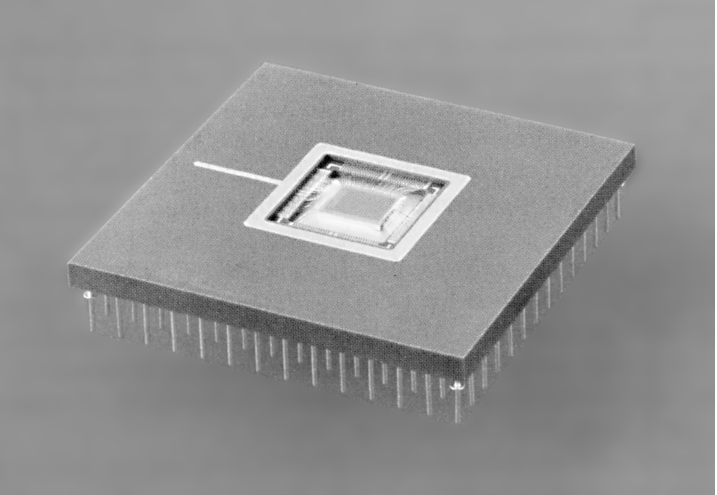
\includegraphics[width=0.8\textwidth]{scalony.png}
\centering
\caption{Sieć neuronowa zrealizowana w formie układu scalonego. Liczba neuronów samej sieci wynosi 16 x 16 = 256. Układ zawiera około 60 000 tranzystorów \citep[s. 14]{Kosinski2017} i \citep{Chua1998}.}
\centering
\end{center}
\end{figure}

Jak do tej pory sztuczne sieci neuronowe wykorzystywano do realizacji wielu skomplikowanych zadań. Jednym z najważniejszych zastosowań jest wykorzystanie sztucznych sieci neuronowych do rozpoznawania obiektów występujących na obrazie. Mogą być to obrazy różnego rodzaju - na przykład tę przedstawiające pismo odręczne (zob. rys 1.2). Sieci neuronowe są również szeroko wykorzystywane do rozwiązywania różnego rodzaju problemów optymalizacyjnych czy do przewidywania ruchów inwestorów na giełdzie \citep[s. 15]{Kosinski2017}.

\begin{figure}[H]
\begin{center}
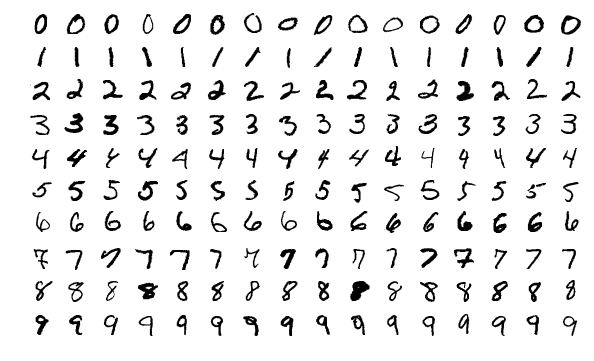
\includegraphics[width=\textwidth]{MINST.png}
\caption{Baza danych \textit{MNIST} zawiera skany odręcznych cyfr, które są powszechnie wykorzystywane w procesie uczenia różnych systemów przetwarzania obrazu. Źródło: \href{https://en.wikipedia.org/wiki/MNIST_database}{Wikipedia}}
\centering
\end{center}
\end{figure}

Sieci neuronowe -- zarówno te biologiczne jak ich sztuczne odpowiedniki -- są systemem złożonym. Mają one właściwości charakterystyczne dla sieci typu \textit{małego świata}. To znaczy, że najkrótsza droga $L$ między dwoma neuronami sieci jest stosunkowo krótka, a prawdopodobieństwo $P$ tego, że neuron ma $k$ sąsiednich neuronów, z którymi jest połączony jest wprost proporcjonalne do wartości $k^{-\Upsilon}$, gdzie stała wartość $2 < \Upsilon < 3$ -- zależy od architektury sieci neuronowej. Na rysunku 1.3 przedstawiono kilka przykładów takich architektur (Za: \citep[s. 15-16]{Kosinski2017}).

\begin{figure}[H]
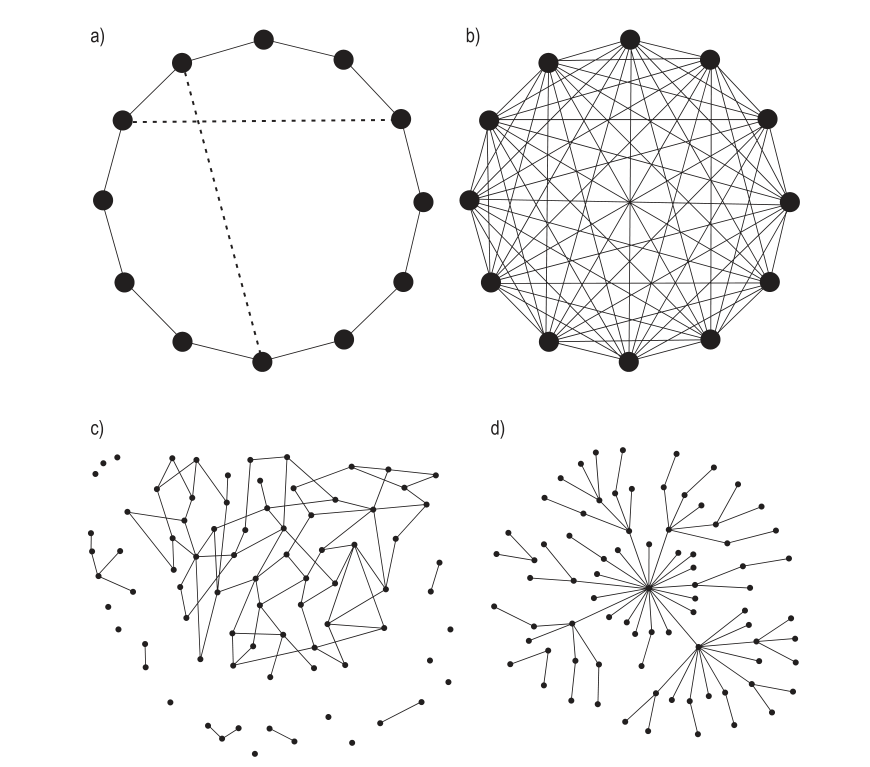
\includegraphics[width =\textwidth]{architektura.png}
\centering
\caption{(a) sieć jednowymiarowa z połączeniami bliskozasięgowymi (linie ciągłe) oraz z połączeniami typu \textit{małego swiata} (linie przerywane (b) sieć całkowicie połączona o 12 węzłach (c) sieć przypadkowo połączona (graf przypadkowy) (d) sieć bezskalowa\protect\footnotemark}
\centering
\end{figure}

\footnotetext{Sieć, w której rozkład liczby połączeń między węzłami jest zgodny z rozkładem \textit{Yule-Simona:}
P(k)\textasciitilde $k^{-\Upsilon}$. \\ gdzie $\Upsilon$ jest parametrem właściwym dla danej sieci i przyjmuje wartości z zakresu (2,3)  Źródło: \href{https://en.wikipedia.org/wiki/Scale-free_network}{Wikipedia}}

\clearpage
\section{Poznanie a rozpoznanie}
Problem automatycznego rozpoznawania obiektów będę tutaj rozpatrywać bazując na idei podziału przestrzeni wyników na rozłączne zbiory (klasy). Wyróżnione zbiory powinny określać wartości wyników obserwacji właściwe poszczególnym obiektom badanego zbioru. \textit{Wynik obserwacji} przedstawia zaobserwowane lub zmierzone wartości cech danego obiektu \citep[s. 7]{Kwiatkowski2007}.

Przez \textit{przestrzeń wyników obserwacji} rozumiemy to samo co pod przestrzenią cech obiektu. Wynik obserwacji stanowi formalnie punkt przestrzeni cech.\footnote{Zakładamy tutaj, że badany przez nas wzór obiekt jest reprezentowany poprzez wektor liczb zwany wartościami cech. Przestrzeń na płaszczyźnie która zawiera wektory cech badanego obiektu nazywamy właśnie przestrzenią cech.} \textit{Rozpoznanie obiektu} polega zatem na obserwacji (pomiarze wartości) cech obiektu i~sprawdzeniu do której klasy w przestrzeni cech zaobserwowany wynik należy. Taki sposób wnioskowania jest charakterystyczny dla zadania \textit{klasyfikacji} \citep[s. 7]{Kwiatkowski2007}.

Podstawowym problemem jest sposób, w jaki dokonamy tego podziału przestrzeni na podstawie dostępnych danych. Kluczem do uzyskania satysfakcjonujących wyników może być sformułowanie we właściwy sposób zadania aproksymacji. Dzięki temu możliwe staje się wykorzystanie metody najmniejszych kwadratów do rekurencyjnego uzyskiwania rozwiązań. Taki sposób postępowania leży u podstaw działania sztucznych sieci neuronowych. Na bazie tego typu sieci zadania poznawania (uczenia się) i rozpoznawania uzyskują naturalną interpretacje \citep[s. 7-8]{Kwiatkowski2007}.

Ujmując problem bardziej ściśle, poprzez rozpoznanie rozumiem wyróżnienie przedmiotu spośród innych występujących w analizowanym zbiorze obiektów. Poznanie zwykle oznacza zdobywanie wiedzy o czymś, nauczenie się czegoś na podstawie doświadczenia. Proces poznawania będę tutaj utożsamiać z uczeniem się.
Wyróżniamy dwa sposoby uczenia się:

\begin{enumerate}[leftmargin=2\parindent] % do wciecia
    \item Uczenie się z nauczycielem (nadzorowane),
    \item Uczenie się bez nauczyciela (nienadzorowane)
\end{enumerate}

Uczenie z nauczycielem polega na wstępnym określeniu cech charakterystycznych dla każdego badanego obiektu: nauczyciel przedstawia wynik obserwacji cech wraz z określeniem właściwego rodzaju obiektu (właściwego wyniku klasyfikacji obiektu). Nauczenie polega na określeniu w przestrzeni cech zbioru wartości właściwych danego obiektu. Rezultatem uczenia jest określenie podzbiorów przestrzeni cech charakteryzujących poszczególne obiekty \citep[s. 8]{Kwiatkowski2007}.

Sposób drugi polega na grupowaniu tych obserwacji, które powodują taką samą reakcje programu dokonującego klasyfikacji. Należy zaznaczyć, że nie zawsze dochodzi tutaj do znalezienia relacji przyczynowo-skutkowej -- często obserwacje są kojarzone w jedną grupę na podstawie innych, często nieintuicyjnych cech obiektów.
Jeśli wyróżnione podzbiory tworzą podział przestrzeni cech (tzn. są rozłączne i wyczerpują całą badaną przestrzeń), to dzięki uzyskaniu odpowiednich klas abstrakcji (grup) możemy zdefiniować nowe obiekty w taki sposób, że każda z dostępnych klas definiuje obiekt \citep[s. 8-9]{Kwiatkowski2007}.

\section{Model sztucznego neuronu}
Jednym z najprostszych modeli sieci neuronowych jest \textbf{sztuczny neuron}. Pojedyncze sztuczne neurony to modele obliczeniowe, które zapoczątkowały rozwój uczenia maszynowego \citep[s. 39]{Raschka_2019}.
Model sztucznego neuronu został zainspirowany -- jak nazwa wskazuje -- neuronem biologicznym, który został przedstawiony na rysunku 1.4.
\begin{figure}[H]
\begin{center}
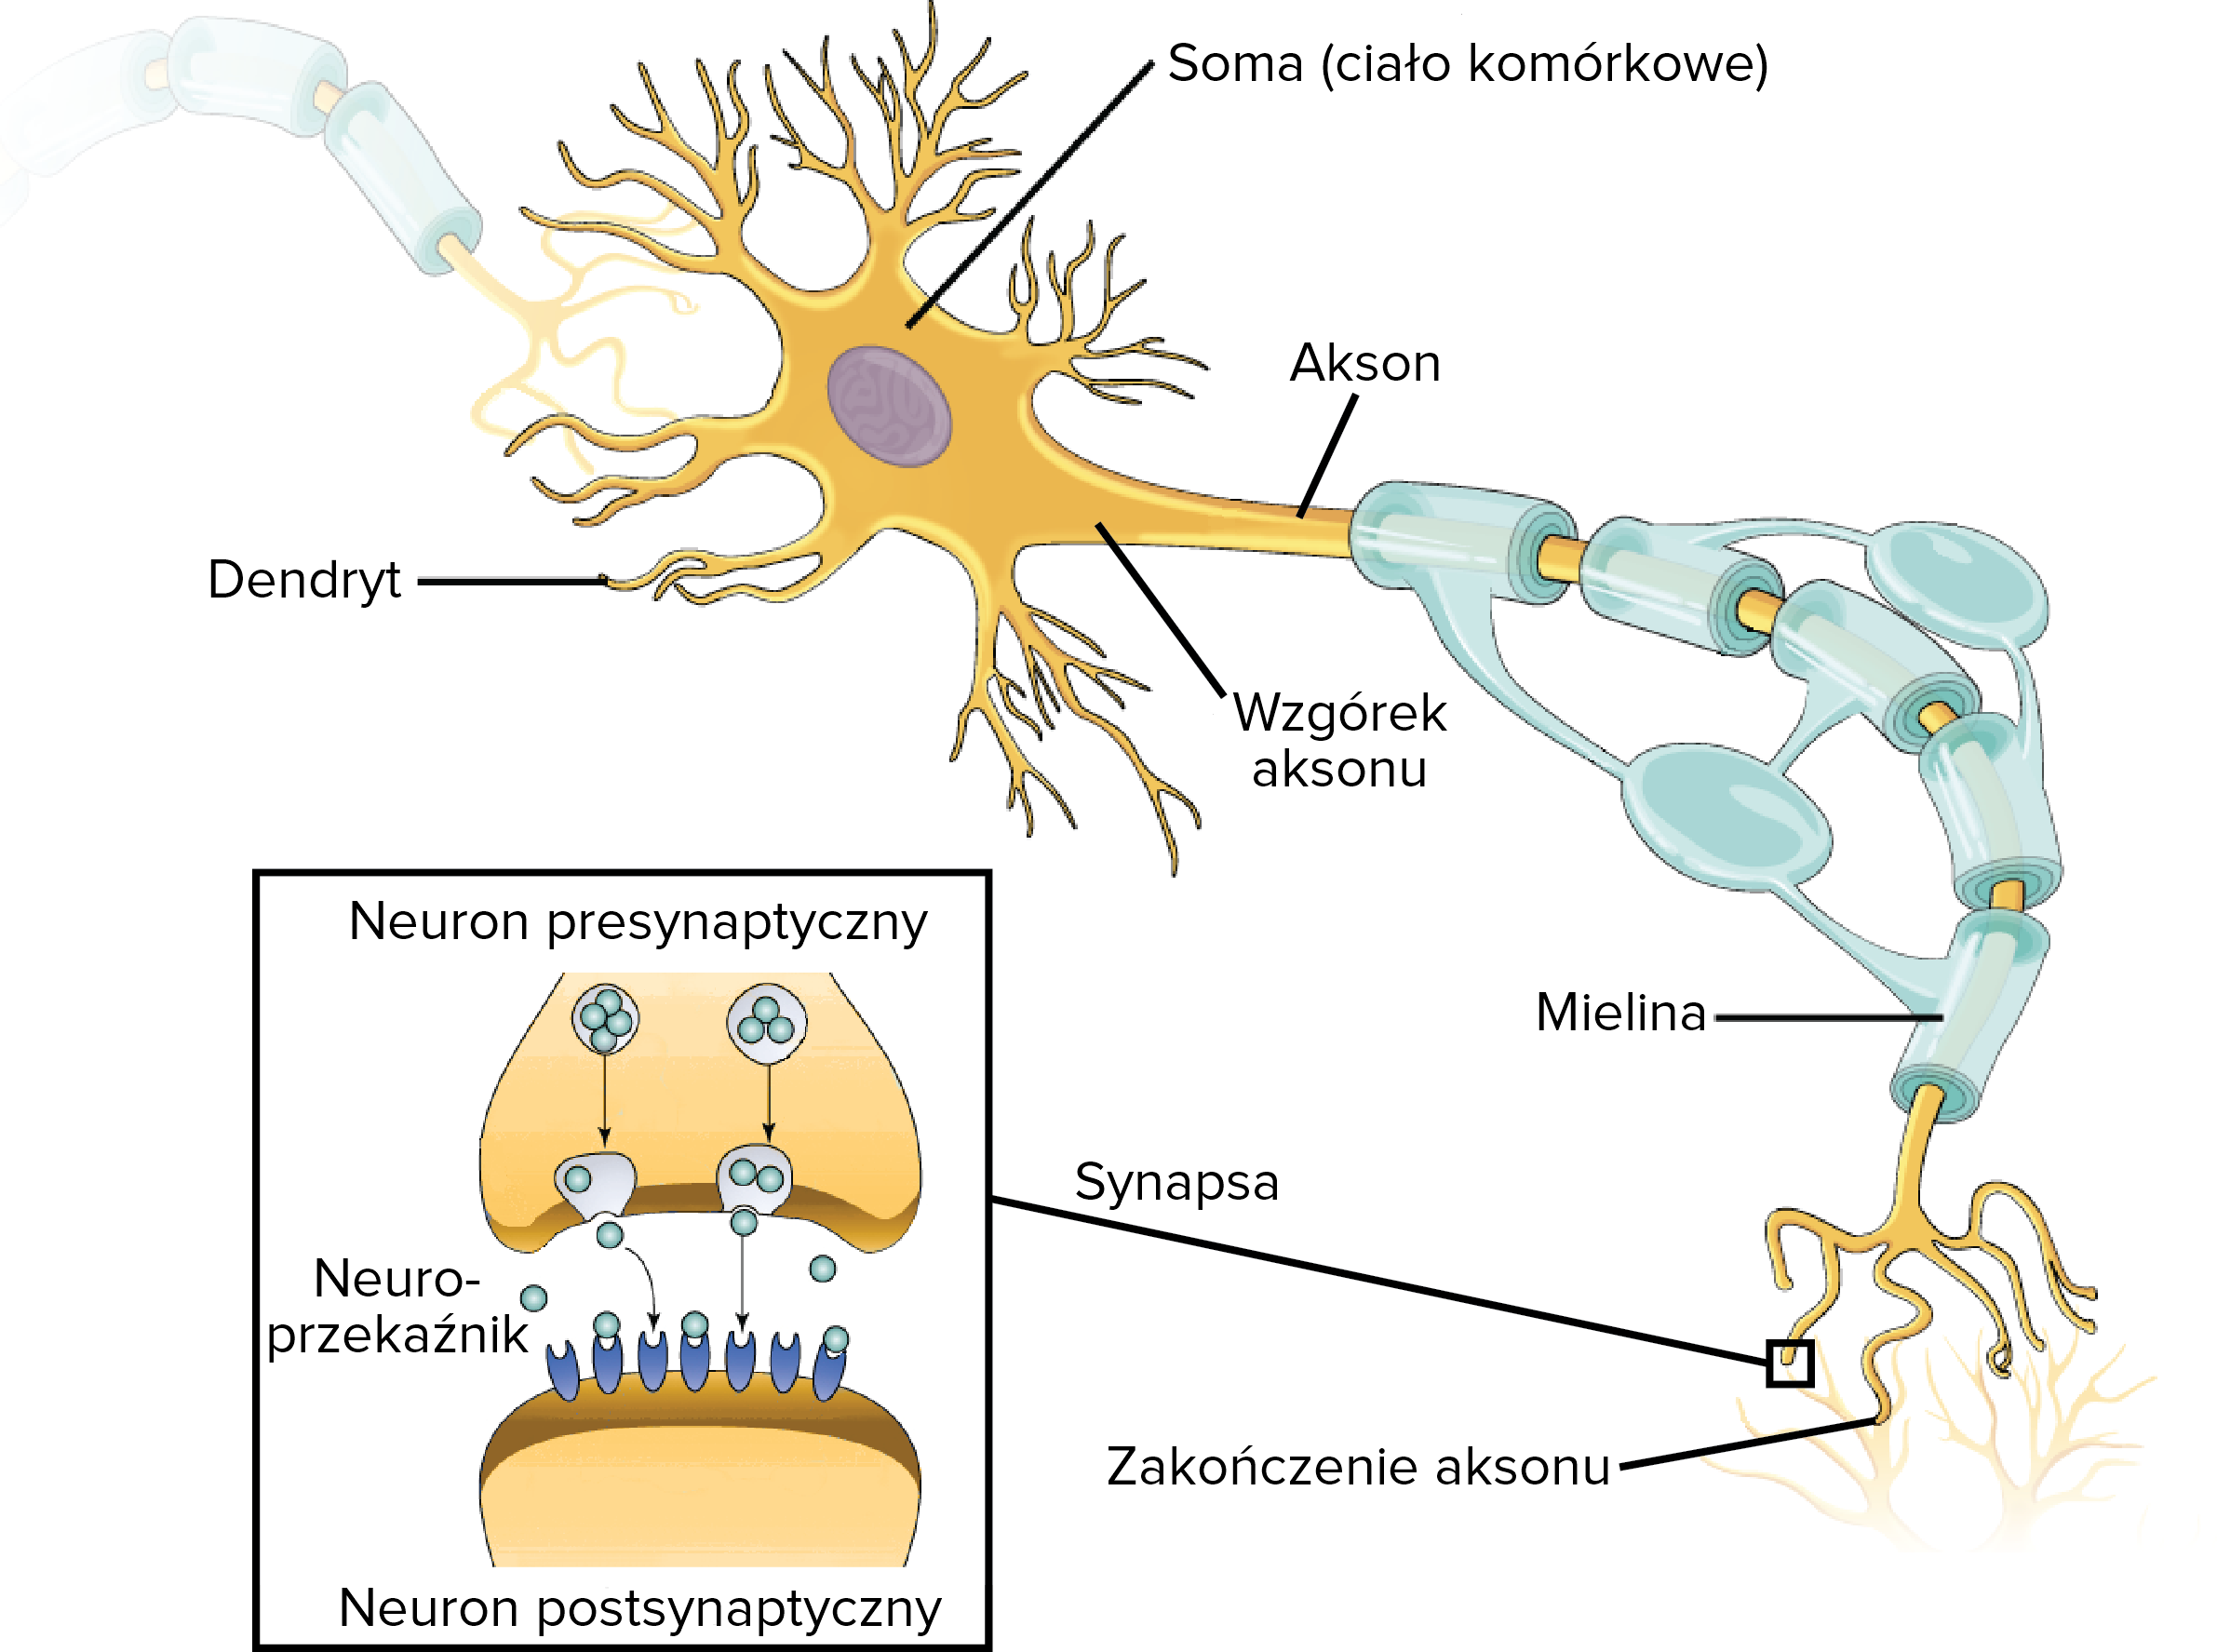
\includegraphics[width=0.8\textwidth]{neuron.png}
\caption{Model neuronu biologicznego. Źródło: \href{https://pl.khanacademy.org/science/biology/human-biology/neuron-nervous-system/a/overview-of-neuron-structure-and-function}{Khan Academy}}
\centering
\end{center}
\end{figure}

Jedną z pierwszych prób formalnego zdefiniowania zasady działania neuronu biologicznego podjeli w roku 1943 \textit{McCulloch} i \textit{Pitts}. Zaproponowali oni pierwszy model sztucznego neuronu tzw. \textbf{Neuron McCullocha-Pittsa} (zob. Rys. 1.5).

McCulloch i Pitts opisali neuron jako bramkę logiczną zawierającą binarne wyjścia. Zasada działania tego modelu jest prosta: do neuronu dociera wiele sygnałów, które po integracji w ciele komórki generują sygnał na wyjściu, jeżeli zostanie przekroczona odgórnie ustalona wartość graniczna. Jeśli coś takiego nie będzie miało miejsca -- neuron nie wygeneruje odpowiedzi na wyjściu \citep[s. 40]{Raschka_2019}.
\begin{figure}[H]
\begin{center}
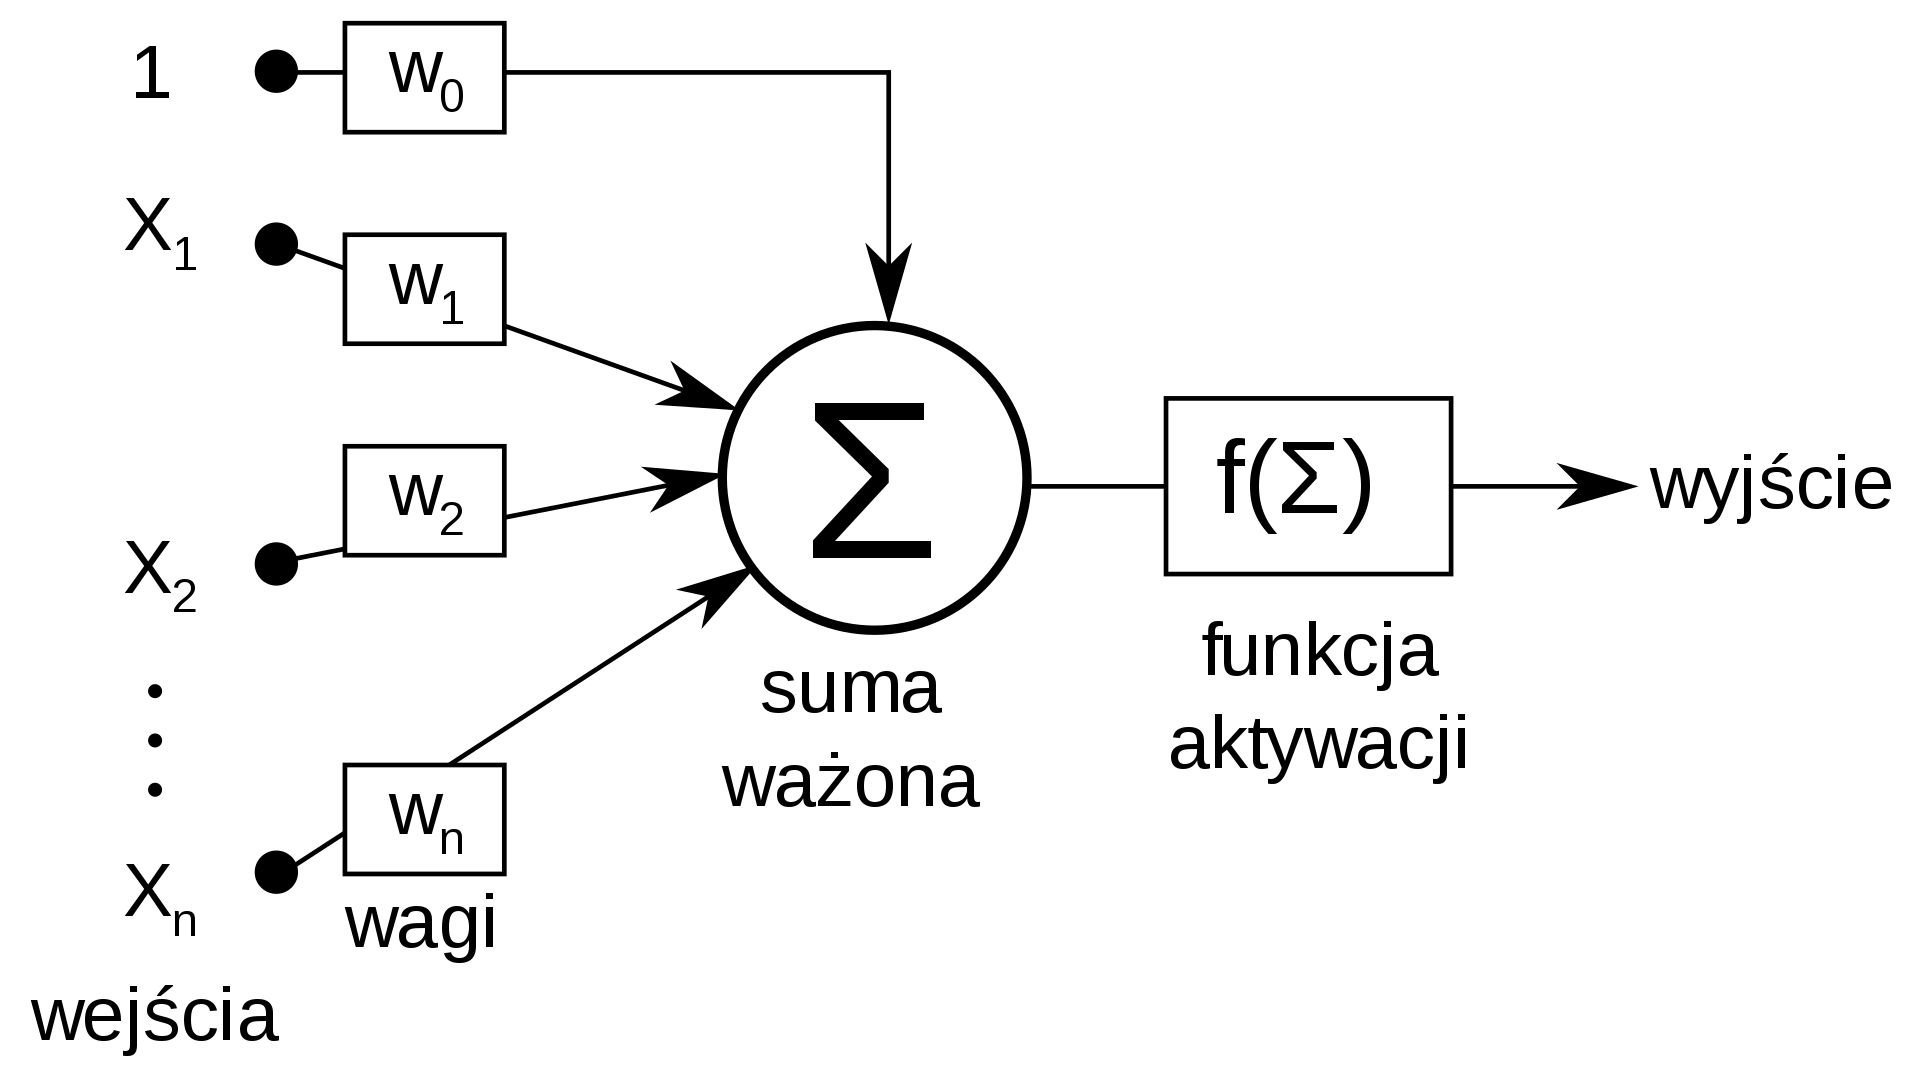
\includegraphics[width=0.8\textwidth]{Pitts.png}
\caption{Model neuronu McCullocha-Pittsa. Jeśli wartość sumy ważonej przekroczy wartośc progową funkcji aktywacji, to zostanie wygenerowana odpowiedź neuronu na wyjściu komórki. Źródło: \href{https://pl.wikipedia.org/wiki/Neuron_McCullocha-Pittsa}{Wikipedia}}
\centering
\end{center}
\end{figure}
Innym przykładem jest \textbf{Perceptron Rosenblatta}. Frank Rosenblatt zaproponował algorytm zdolny do automatycznego uczenia się za pomocą optymalnych współczynników wag, które są przemnażane przez wartości obecne na wejściu neuronu, co pozwala w jednoznaczny sposób określić czy neuron ma przekazać dalej otrzymany sygnał. W kontekście uczenia nadzorowanego można wykorzystać ten mechanizm do realizacji zadania klasyfikacji obiektu do różnych klas \citep[s.40]{Raschka_2019}.

\section{Cel pracy}

Celem pracy nie jest opis konkretnej implementacji sieci neuronowej ani zaprojektowanie takiej sieci od podstaw. Celem, który zamierzamy zrealizować w niniejszej pracy jest  zastosowanie pewnych cech i funkcji typowych dla sieci neuronowej do realizacji zadania kompozycji dzieła muzycznego. Sieć neuronowa jest mechanizmem opracowanym do rozpoznawania pewnych wzorców w danych i podejmowaniu na ich podstawie konkretnych decyzji lub tylko sugerowaniu pewnych rozwiązań właściwym decydentom. Te właściwość sieci zamierzamy właśnie wykorzystać. Planujemy zbudować system, który właściwie rozpozna cechy dzieła muzycznego i będzie w stanie je uogólnić do rozpoznawania ich  w szerszej klasie przykładów (zadanie klasyfikacji). Dodatkowo chcemy aby system dysponował zdolnością do tworzenia nowego utworu muzycznego na podstawie gotowego przykładu (zadanie generowania muzyki). Do realizacji tego zadania skorzystamy z pewnych cech, które zwyczajowo w literaturze przypisuje się właśnie sztucznym sieciom neuronowym.   

\chapter{Podstawy aparatu matematycznego algebry liniowej}

Nasze rozważania na temat modelowania dzieła muzycznego należy rozpocząć od zdefiniowania problemu w sposób formalny i wprowadzeniu podstawowych pojęć z zakresu niezbędnego aparatu matematycznego używanego do opisu i projektowania sieci neuronowych oraz do wprowadzenia pewnych podstawowych pojęć z zakresu teorii muzyki, których zdefiniowanie jest konieczne w celu prowadzenia dalszych rozważań. Realizacji tych dwóch zadań są poświęcone następne dwa rozdziały niniejszej pracy.

\section{Grupa abelowa}
\begin{definicja}
Niech V będzie niepustym zbiorem wraz z zdefiniowanym działaniem wewnętrznym +. Zbiór $(V,+)$ jest \textbf{grupą abelową} jeśli spełnia on poniższe warunki\footnote{Za: \url{http://en.math.uni.lodz.pl/~wiertelak/Temat20.pdf}}:
\end{definicja}

\begin{equation*}
 \forall_{u,w,v \in V} \quad (u + w) + v = u + (w + v) \quad \text{(łączność)}
\end{equation*}

\begin{equation*}
 \exists_{e \in V}, \quad \forall_{a \in V} \quad a  + e = e + a = a \quad \text{(element neutralny)}
 \end{equation*}
 
 \begin{equation*}
     \exists_{a \in V}, \quad \forall_{a^{-1} \in V} \quad 
     a + (-a) = e + (-a) + a = e \quad \text{(elementy odwrotne)}
 \end{equation*}
 
 a ponadto jeśli poniższe działanie jest przemienne to grupa jest grupą abelową.
 
\begin{equation*}
    \forall_{u,w \in V} \quad u + w = w + u
\end{equation*}

\section{Przestrzenie wektorowe}

Czwórkę postaci (V;$\mathbb{R}$;+;$\cdot$), gdzie V jest zbiorem nad ciałem $\mathbb{R}$, + jest działaniem wewnętrznym w zbiorze V oraz $\cdot$ jest mnożeniem elementów zbioru V przez elementy ciała $\mathbb{R}$ nazywamy \textit{przestrzenią wektorową}, jeśli spełnione są następujące warunki:
\begin{axioms}
\item \label{} (V; +) jest grupą abelową,
\item \label{item:L2} \quad $\bigwedge_{a \in R^{n}}, \bigwedge_{v, w \in V} \quad  a(v+w) = av +aw$,
  
  \item \label{item:L3} $\bigwedge_{a,b \in R^{n}}, \bigwedge_{v \in V} \quad  (a + b)v = av + bv$,
  
  \item \label{item:L4} $\bigwedge_{a,b \in R^{n}}, \bigwedge_{v \in V} \quad  a(bv) = (ab)v$, 
  
  \item \label{item:L5} $\bigwedge_{v \in V} \quad  1v = v$.
  
\end{axioms}

Poszczególne elementy zbioru V nazywamy \textit{wektorami}, a elementy przestrzeni nad ciałem $\mathbb{R}$ nazywamy \textit{skalarami}. Zbiór wektorów V nazywamy \textit{rzeczywistą przestrzenią wektorową} \citep[s. 27]{Rutkowski_2008}.




Zdefiniujmy zbiór wektorów V nad ciałem $\mathbb{R}$ gdzie, $v,w \in V$ i są one następującej postaci:
\begin{equation*}
V = \{v: v = [v_{1},\cdots, v_{n}], \quad v_{i} \in R, \quad i = 1,\cdots,n\}.
\end{equation*}
Dla $v,w \in V$ w zbiorze $v$ możemy następnie wprowadzić operacje dodawania:
\begin{equation*}
    v + w = [v_{1}, \cdots, v_{n}] + [w_{1}, \cdots, w_{1}] 
    = [v_{1} + w_{1}, \cdots, v_{n} = w_{n}].
\end{equation*}
Oznaczmy
\begin{equation*}
    -v = -[v_{1},\cdots,v_{n}] = [-v_{1},\cdots,-v_{n}]
\end{equation*}
jako element przeciwny do wektora v. Mamy zatem
\begin{equation*}
    v + (-w) = [v_{1},\cdots,v_{n}] + [-w_{1},\cdots,-w_{n}]
    = [v_{1}-w_{1},\cdots,v_{n}-w_{n}]
\end{equation*}
Definiujemy element neutralny dodawania $\Theta$ postaci:

\begin{equation*}
    \Theta = [0,\cdots,0]
\end{equation*}
Wprowadzimy operacje mnożenia wektora przez liczbę rzeczywistą $a \in \mathbb{R}$ (skalar) następującej postaci:
\begin{equation*}
a \cdot v = a[v_{1}, \cdots, v_{n}] = [av_{1},\cdots, av_{n}].
\end{equation*}
Zdefiniowany powyżej zbiór $V$ wraz z operacją dodawania wektorów tworzy grupę abelową, a wraz z mnożeniem przez skalar jest przestrzenią liniową nad $\mathbb{R}$.

\section{Iloczyn skalarny i przestrzenie unitarne}

\begin{definicja}\footnote{Definicje opracowano na podstawie: \citep[s. 198]{Rutkowski_2008}.}
Niech V będzie przestrzenią wektorową nad ciałem $\mathbb{R}$. Iloczynem skalarnym w przestrzeni V nazywamy funkcję $\big \langle \cdot, \cdot \big \rangle$: V x V $\rightarrow \mathbb{R}$ spełniającą warunki:
\\
\begin{axioms}
    \item $\bigwedge_{v,w \in V} \big \langle v, w \big \rangle = \overline{\big \langle v, w \big \rangle}$,
    
    \item $\bigwedge_{a,b \in R} \bigwedge_{v_{1},v_{2} \in V} \big \langle av_{1} + bv_{2}, w \big \rangle = a \big \langle v_{1}, w \big \rangle + b \big \langle v_{2}, w \big \rangle$,
    \item $\bigwedge_{v \in V \backslash \{\theta\}} \big \langle v, v \big \rangle > 0$. 
\end{axioms}
\end{definicja}

Przestrzenią unitarną nazywamy parę (V, $\big \langle \cdot, \cdot \big \rangle$), gdzie V jest przestrzenią wektorową, a $\big \langle \cdot, \cdot \big \rangle$ jest iloczynem skalarnym w przestrzeni V.
Jeśli wiadomo jaki iloczyn skalarny został określony w przestrzeni V, to samą przestrzeń V nazywamy \textit{przestrzenią unitarną} \citep[s. 198-199]{Rutkowski_2008}.
\newline
Iloczyn skalarny ma następujące własności:
\begin{axioms}
\item $\bigwedge_{v \in V} \quad \big \langle v, \theta \big \rangle =  \big \langle \theta, v \big \rangle = 0$,

\item $\bigwedge_{v \in V} \quad \big \langle v, v \big \rangle \geq 0$,
\item $\bigwedge_{v,w_{1},w_{2} \in V} \quad \big \langle v, w_{1} + w_{2} \big \rangle =  \big \langle v, w_{1} \big \rangle + \big \langle v, w_{2} \big \rangle$,
\item $\bigwedge_{a in R} \quad \bigwedge_{v, w \in V} \quad \big \langle v, aw \big \rangle = \overline{a} \big \langle v, w \big \rangle$.

\end{axioms}

\begin{definicja}
Niech V będzie przestrzenią unitarną. Normą(długością) wektora $v \in V$ nazywamy liczbę rzeczywistą nieujemną $\sqrt{\big \langle v, v \big \rangle}$. Normę wektora v oznaczamy przez $\|v\|$. Wektor $v \in V$ nazywamy wektorem \textit{unormowanym}, jeżeli $\|v\| = 1$.
\end{definicja}

Jeśli V jest przestrzenią unitarną nad ciałem $R^{n}$, to dla dowolnie wybranych $a \in R$ i $v \in V$ zachodzi dodatkowo następująca równość:
\begin{equation*}
   \|av\| = |a| \ \|v\|
\end{equation*}

Dodatkowo, jeśli V jest przestrzenią unitarną, to dla dowolnych wektorów $v,w \in V$ zachodzą ponadto nierówności:
\begin{figure}[H]
\begin{equation*}
    |\big \langle v, w \big \rangle| \ \leqq \ \|v\| \cdot \|w\| \quad \text{(nierówność Schwarza)}
\end{equation*}

\begin{equation*}
    \|v + w\| \ \leqq \ \|v\| + \|w\| \quad \text{(nierówność Minkowskiego)}
\end{equation*}

\begin{equation*}
    \Bigg| \|v\| - \|w\| \Bigg| \ \leqq \ \|v - w \|.
\end{equation*}
\end{figure}

\section{Proste zadanie klasyfikacji}

W tym podrozdziale przedstawimy rozumowanie, którego celem  jest pokazanie czytelnikowi w jaki sposób można, na poziomie ogólnym, zbudować prosty układ klasyfikujący obiekty.\footnote{Opracowane na podstawie: \citep[s. 11]{Kwiatkowski2007}} Układ ten będzie prostym klasyfikatorem binarnym, przydzielającym obiekty do dwóch niezależnych klas, a zasada jego działania będzie zbliżona, ale prostsza od zasady działania wspomnianego wyżej perceptronu.
\\

Ustalmy, że $u, v \in \mathbb{R}^{n}$:
\begin{equation*}
    u = \big[u_{1},\cdots,u_{n}\big] \qquad v = \big[v_{1},\cdots,v_{n}]
\end{equation*}

Niech $u$ i $v$ będą wyróżnionymi punktami przestrzeni $\mathbb{R}^{n}$. Zdefiniujmy na niej klasę $\bm{C}^{(1)}$ punktów w przestrzeni $R^{n}$ jako zbiór punktów położonych bliżej punktu $u$ niż $v$:

\begin{equation}
    \bm{C}^{(1)} = \bigg\{ x \in \mathbb{R}^{n} : \| x - u\| < \| x - v\| \bigg\} 
\end{equation}

Analogicznie określimy klasę $\bm{C}^{(2)}$ jako zbiór punktów bliższych punktowi $v$:

\begin{equation}
    \bm{C}^{(2)} = \bigg\{ x \in \mathbb{R}^{n} : \|x - v\| < \| x - u\| \bigg\}
\end{equation}
Punkty $\bm{u}$ i $\bm{v}$ rozumieć będziemy jako wzorce wartości cech odpowiednich obiektów. Przyporządkowanie badanego punktu $\bm{x}$ przestrzeni cech $\mathbb{R}^{n}$ do jednej z dwóch klas stanowi dość prosty przykład realizacji zadania rozpoznania obiektu.

Kolejny krok polega na wyznaczeniu granic dla klas $\bm{C}^{(1)}$ i $\bm{C}^{(2)}$. 
\\
Niech:

\begin{equation}
\|{x - v}\| = \|{x- u}\|
\end{equation}

więc
\begin{equation}
    \big \langle x - v | x - v \big \rangle = \big \langle x - u | x - u \big \rangle.
\end{equation}

Zatem,

\begin{equation*}
    \big \langle x - v | x - v \big \rangle = \big \langle x - v |x \big \rangle - \big \langle x - v | v \big \rangle = \big \langle x | x \big \rangle - \big \langle x | v \big \rangle - \big \langle x | v \big \rangle + \big \langle v | v \big \rangle = \|x\|^{2} + \|v\|^{2} - 2 \big \langle x | v \big \rangle 
\end{equation*}

oraz
\begin{equation*}
    \big \langle x - u | x - u \big \rangle = \|x\|^{2} + \|u\|^{2} - 2 \big \langle x | u \big \rangle.
\end{equation*}

Stąd,
\begin{equation}
    \frac{1}{2} \big( \|v\|^{2} - \|u\|^{2} \big) = \big \langle x|v \big \rangle - \big \langle x|u \big \rangle = \big \langle x|v - u \big \rangle = \big \langle v - u|x \big \rangle.
\end{equation}

Niech $y = v - u$ oraz $w_{0} = \frac{1}{2} \bigg(\|v\|^{2} - \|u\|^{2}\bigg).$ 

Wtedy:

\begin{equation*}
\bm{\big \langle y|x \big \rangle = w_{0}}.
\end{equation*}

Na tej podstawie możemy zdefiniować funkcje klasyfikującą:

\begin{equation}
f(x) =\left\{\begin{matrix}
1, & dla  & \big \langle y|x \big \rangle > w_{0} \\ 
-1,& dla & \big \langle y|x \big \rangle < w_{0}  
\end{matrix}\right.
\end{equation}

Stąd,

\begin{equation}
\left\{\begin{matrix}
x \in C_{1}, & dla  & f(x) = 1 \\ 
x \in C_{2},& dla & f(x) = -1
\end{matrix}\right.
\end{equation}
\\
\begin{przyklad}
Chcemy zaklasyfikować wektor $x$ do którejś z klas $C_{1}$ lub ${C_{2}}$.
\\

\begin{equation*}
v = [1,2]  \qquad u =[3, -5] \qquad x = [2,4]
\end{equation*}
Otrzymujemy kolejno:
\begin{equation}
    y =  v - u = [1 - 3 , 2 -(-5)] = \textbf{[-2,7]}.
\end{equation}
\begin{align}
       w_{0} = &  \frac{1}{2} \big(\|v\|^{2} - \|u\|^{2}\big)  \\ 
        = &\frac{1}{2}((1 \cdot 1 + 2 \cdot 2) - (3 \cdot 3 + (-5) \cdot (-5))  \\
        = & \frac{1}{2}((1 + 4) - (9 + 25))   \\
       = &\frac{1}{2}(5 - 34) = \frac{1}{2} \cdot -29 = \textbf{-14,5}.
    \end{align}


Wtedy
\begin{equation}
    \big \langle y|x  \big \rangle = [-2,7] \cdot [2,4]
    = [-2 \cdot 2 + 7 \cdot 4] = -4 + 28 = \textbf{24}.
\end{equation}

\begin{center}
Jeśli $ \big \langle y|x \big \rangle > w_{0}$ (\textbf{24 > -14,5}), więc otrzymujemy 1.
\end{center}

Zatem z definicji funkcji $f(x) = 1$ wynika, że powinniśmy zaklasyfikować wektor $x$ do klasy $C_{1}$.
\end{przyklad}
\chapter{Podstawy teorii muzyki i formatu MIDI} 
Zanim przejdziemy do omawiania poszczególnych części z jakich składa się utwór muzyczny. Należy wyjaśnić jedną zasadniczą kwestie - Muzyka istniała na tysiące lat zanim pojawiła się teoria ją opisująca.
Koncepcje i reguły składające się na teorie muzyki są w zasadzie podobne do reguł jakie stosuje się w języku naturalnym. Podobnie jak opanowanie gramatyki, pozwala na swobodne prowadzenie konwersacji, tak opanowanie reguł tworzenia muzyki pozwala lepiej tworzyć własne kompozycje i czytać cudze \citep[s. 22]{Pilhofer2018}.

Wiele osób uważa, że teoria muzyki powstała w starożytnej Grecji, ale pierwsze instrumenty muzyczne, zdaniem historyków, powstały już około 7000 lat p.n.e. W okresie formowania się pierwszych osad ludzkich, na długo przed Starożytną Grecją. Na niektórych replikach fletów z kości słoniowej, które powstały w tamtym okresie nadal da się tworzyć utwory muzyczne. Fakt ten nie umniejsza oczywiście osiągnięciom Greków - Pitagoras z Samos stworzył dwunastodźwiękową przypominająca tą, której muzycy używają współcześnie. Stworzył także pierwsze \textit{koło kwintowe}.\footnote{Jest to rodzaj schematu pozwalający opisać pokrewne tonacje poszczególnych dźwięków.} W istocie wkład starożytnych Greków w muzykę był na tyle znaczny, że przez dłuższy czas nie wprowadzano do niej żadnych znacznych modyfikacji \citep[s. 23]{Pilhofer2018}.

\section{Podstawy teorii muzyki} 
Wyjaśnienie podstaw teorii muzyki zaczniemy od jej części składowych: \textit{nut, pauz i tempa}.
Tempo (bit) to pulsacja dzieląca czas na równe odcinki. To czym jest bit dobrze uosabia mechanizm działania zegara. Na każdą minutę składa się 60 tyknięć wskazówki sekund, a każde z tych tyknięć to oddzielny bit. Jeśli przyspieszymy lub spowolnimy wskazówkę zegara, to zmienimy \textit{tempo} tyknięć. Rolą nut w muzyce jest przekazywanie informacji o tym co powinno być zagrane w każdej z oddzielnych tyknięć. Innymi słowy mówią one o tym jak długo i jak często powinno się zagrać określoną \textit{wysokość dźwięku} \citep[s. 31]{Pilhofer2018}.

Każda nuta ma budowę trzyczęściową. Składa się z \textit{główki, ogonka} i \textit{chorągiewki}.
\begin{itemize}
 \item Główka to okrągła część nuty, każda nuta ją ma. Cała nuta składa się tylko z główki,
 \item Ogonek to pionowa linia wychodząca od główki. Mają ją \textit{ósemki, ćwierćnuty} i \textit{półnuty},
 \item Chorągiewka to mała linia wychodząca z lub od ogonka. Chorągiewkę ma \textit{ósemka} i każda nuta od niej krótsza \citep[s. 32-33]{Pilhofer2018} (zob. rys. 3.1).
\end{itemize}

\begin{figure}[H]
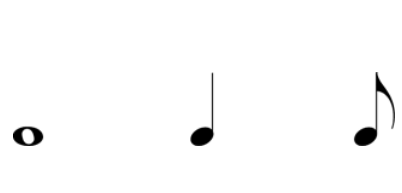
\includegraphics[scale = 0.6]{nuty.png}
\centering
\caption{Od lewej: cała nuta, ćwierćnuta i ósemka. Źródło: \citep[s. 33]{Pilhofer2018}.}
\centering
\end{figure}

Zamiast rysować chorągiewkę przy każdej nucie, można je połączyć \textit{belką}, która trochę upraszcza zapis. (zob. rys. 3.2).

\begin{figure}[H]
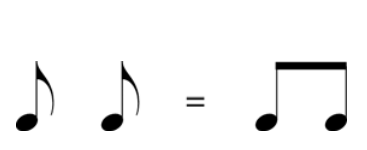
\includegraphics[scale = 0.6]{belka.png}
\centering
\caption{Ósemki można zapisywać oddzielnie lub razem łącząc je za pomocą belki. Źródło: \citep[s. 33]{Pilhofer2018}.}
\centering
\end{figure}
Kolejny rysunek przedstawia szesnastki z chorągiewkami. Sposób zapisu nie ma znaczenia, gdyż wszystkie gra się tak samo (zob. rys. 3.3).
\begin{figure}[H]
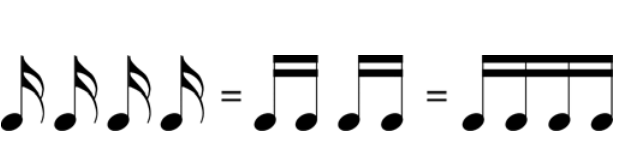
\includegraphics[scale = 0.5]{szesnastki.png}
\centering
\caption{Szesnastki pogrupowane jako: pojedyncze nuty, szesnastki połączone podwójnymi belkami oraz jako grupę nut połączonych jedną podwójną belką. Źródło: \citep[s. 33]{Pilhofer2018}.}
\centering
\end{figure}

Dobrym sposobem na prześledzenie w jaki sposób rozkładają się wartości poszczególnych nut jest skorzystanie z \textit{drzewa nut} pokazanego na rysunku 3.4. 

\begin{figure}[H]
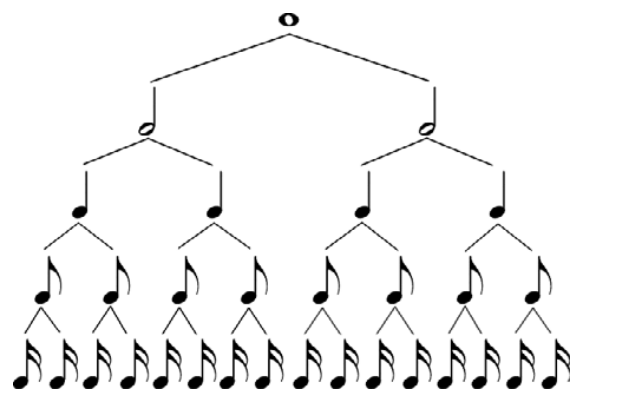
\includegraphics[scale = 0.6]{drzewo.png}
\centering
\caption{Drzewo nut składa się z całej nuty rozkładającej się na dwie półnuty, które następnie rozkładają się na cztery ćwierćnuty. Ćwierć nuty rozkładają się na ósemki, a ósemki na szesnastki Źródło: \citep[s. 34]{Pilhofer2018}.}
\centering
\end{figure}

\textit{Pauza} to cisza w muzyce. Pauzy są szczególnie ważne gdy piszę się utwory, które mają być czytane przez innych ludzi. Pozwalają one na precyzyjniejsze wskazanie rytmu niż za pomocą samych nut. Rysunek 3.5 przedstawia względne wartości pauz. Podobnie jak w drzewie nut na samej górze jest pauza całonutowa, potem półnutowa, ćwierćnutowa, ósemkowa i szesnastkowa \citep[s. 40-41]{Pilhofer2018}

\begin{figure}[H]
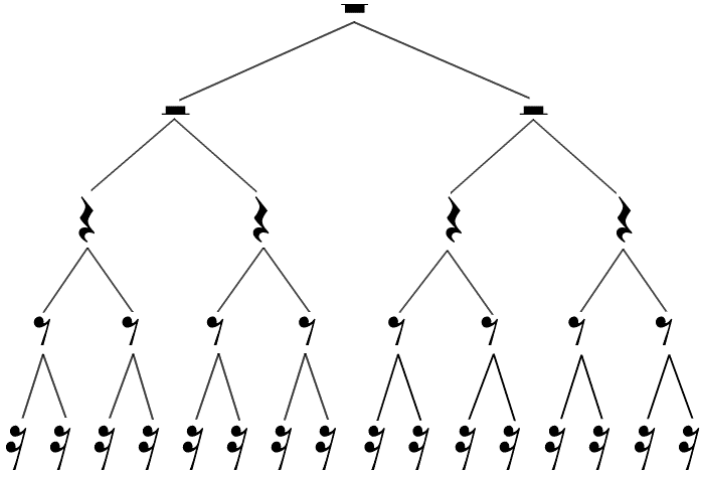
\includegraphics[scale = 0.5]{pauzy.png}
\centering
\caption{Drzewo pauz. Źródło: \citep[s. 42]{Pilhofer2018}.}
\centering
\end{figure}

Nuty i pauzy zapisuje się na \textit{pięciolinii} (zob. rys. 3.6). Pięciolinia składa się z pięciu równoległych poziomych linii i czterech przerw między liniami. Nuty i pauzy umieszczane są na liniach, jak i na przerwach między liniami. Wysokość dźwięku oznaczana przez poszczególne linie i przerwy jest wskazywana przez \textit{klucz} znajdujący się na początku pięciolinii. Istnieją dwa główne rodzaje kluczy:
\begin{enumerate}
    \item klucz wiolinowy -- za jego pomocą oznacza się pięciolinie do zapisu wyższych dźwięków,
    \item klucz basowy -- tego rodzaju pięciolinii używa się do grania niższych dźwięków,
\end{enumerate}

Pięciolinia umożliwia wygodne przedstawienie wysokości dźwięku (zarówno pojedynczo jak i w akordach), z uwzględnieniem czasu ich trwania.
 Każda wysokość lub ton na pięciolinii ma nazwę jednej z siedmiu liter alfabetu: \textit{A,H,C,D,E,F,G,A,H,C}.
 
 \begin{figure}[H]
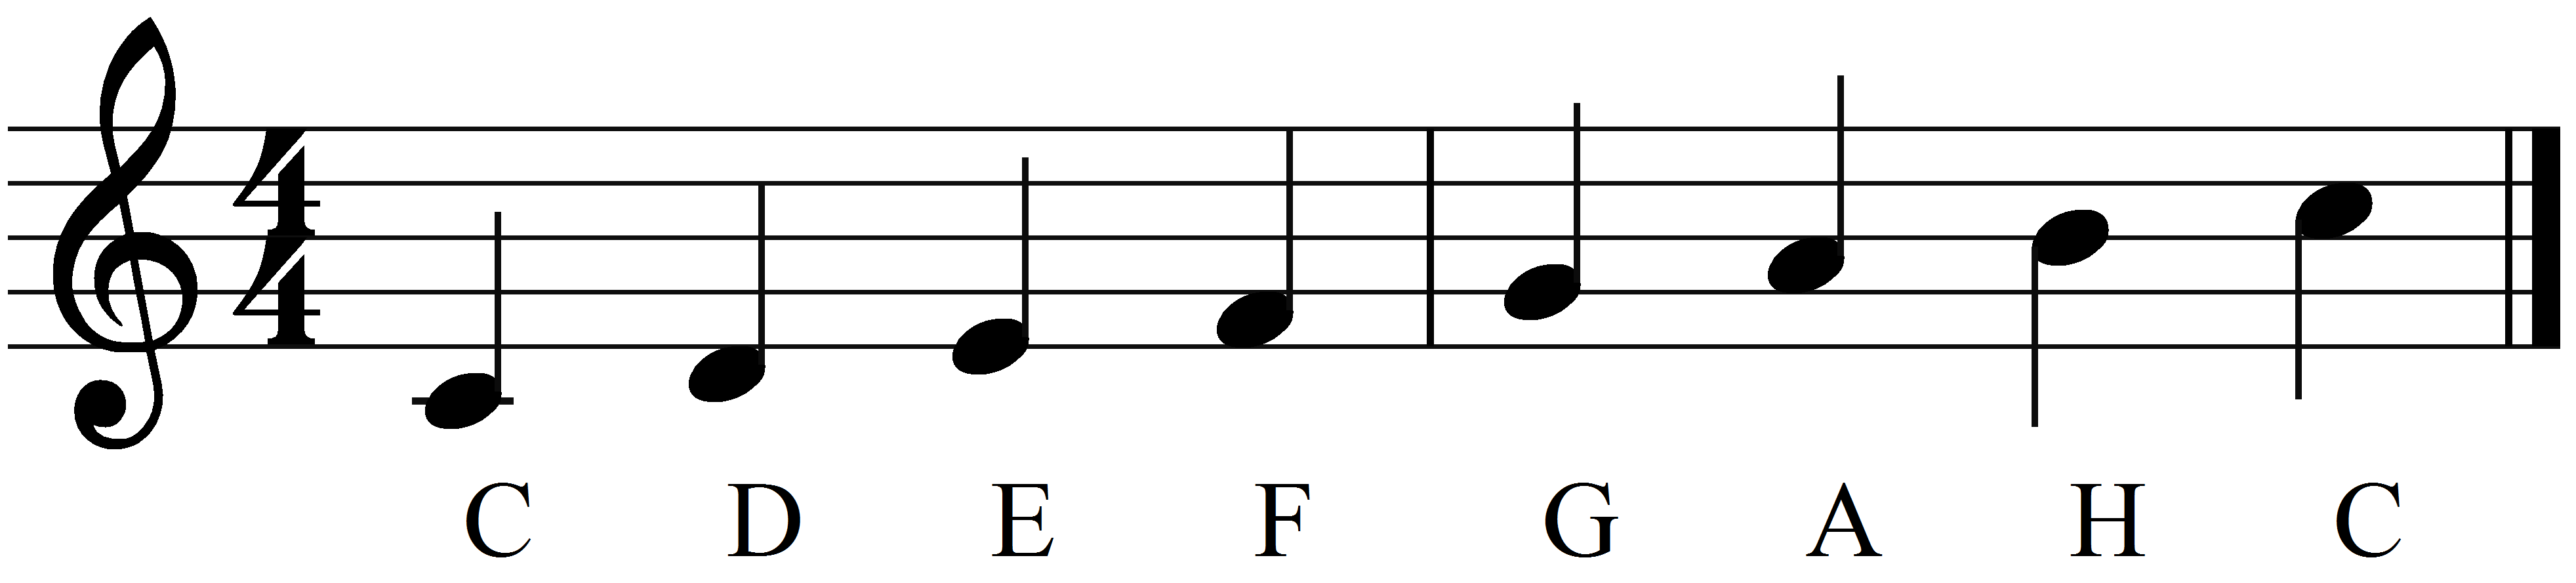
\includegraphics[scale = 0.9]{pieciolinia.png}
\centering
\caption{Gama C-dur. C-dur to tonacja muzyczna oparta na skali durowej. Zawiera siedem dźwięków od A do H(B). Źródło: https://pl.wikipedia.org/wiki/C-dur}
\centering
\end{figure}

Jeśli teoria muzyki to wiedza na temat tego z jakich elementów można stworzyć muzykę, to \textit{kompozycją} nazywamy umiejętność budowania \textit{utworu muzycznego} z tych podstawowych elementów \citep[s. 22]{Usarzewicz2018}.
Poza nutami, tempem i pauzą. Utwór muzyczny składa się także z \textit{interwałów}, \textit{akordów} oraz \textit{skal}.

\textit{Interwał} to inaczej odległość pionowa między dwoma dźwiękami na pięciolinii (zob. rys. 3.7) 

 \begin{figure}[H]
 \centering
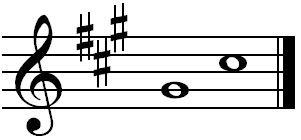
\includegraphics[scale= 0.4]{interwal.png}
\caption{Interwał. Źródło: \citep[s. 22]{Usarzewicz2018}.}
\centering
\end{figure}

\textit{Akord} to współbrzmienie co najmniej trzech dźwięków ułożonych na pięciolinii jeden nad drugim. Akordy są ważnym elementem budującym \textit{harmonie} w utworze. Harmonia zajmuje się łączeniem akordów w większe całości (zob. rys. 3.8) \citep[s. 23]{Usarzewicz2018}.

 \begin{figure}[H]
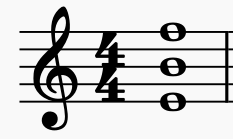
\includegraphics[scale = 0.7]{akord.png}
\centering
\caption{Akord. Źródło: Opracowanie własne w programie MuseScore.}
\centering
\end{figure}

Zestaw następujących po sobie dźwięków, ułożonych w określonej kolejności, to \textit{skala muzyczna}. Najczęściej spotyka się skale \textit{minorową(molową)} i \textit{majorową(durową)} Utwory oparte na skali molowej często uważa się za mające smutne brzmienie. Natomiast utwory oparte o skale durową często uważa się za radosne. Na rysunku 3.9 przedstawiono jedną ze skal, tak zwaną \textit{pentatonikę} \citep[s. 81 - 82]{Pilhofer2018}. 

 \begin{figure}[H]
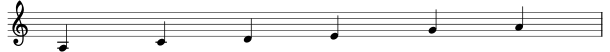
\includegraphics[width=\textwidth]{pentatonika.png}
\caption{Pentatonika z dźwiękiem centralnym D. Pentatonika to jedna z tradycyjnych skal muzycznych, która wywodzi się ze starożytności i jest popularna w muzyce ludowej  Źródło: https://pl.wikipedia.org/wiki/Pentatonika}
\centering
\end{figure}

\section{Format MIDI}
\textit{MIDI} to z języka angielskiego \textit{cyfrowy interfejs instrumentów muzycznych}. Służy on do przekazywania informacji pomiędzy cyfrowymi instrumentami muzycznymi. MIDI umożliwia komputerom, syntezatorom, keyboardom i kartom dźwiękowym komunikowanie się w wspólnym standardzie wymiany informacji oraz pozwala synchronizować się nawzajem. System ten pozwolił także na stworzenie łatwych w obsłudze \textit{sekwencerów} i \textit{syntezatorów perkusyjnych}.

Standard MIDI został stworzony w roku 1983 i znacznie ułatwił pracę z syntezatorami dźwięku. W czasach przed MIDI każdy syntezatorów należało indywidualnie zaprogramować \citep{MIDI}.

W przeciwieństwie do innych formatów audio (jak .flac lub .wav) format MIDI sam w sobie nie przechowuje dźwięku, zawiera jedynie instrukcje jak dany dźwięk zrekonstruować, Jest swoistym rodzajem \textit{cyfrowej pięciolinii} \citep[s. 1 - 2]{MIDI_Format}.
Protokół MIDI pozwala na wysłanie informacji przez maksymalnie 16 różnych kanałów, co pozwala na jednoczesną grę do 16 różnych instrumentów. Można powiedzieć, że standard MIDI specyfikuje zarówno wymagania wstępne względem typu urządzenia mającego odtwarzać dźwięk jak i sam protokół transmisji, według którego mają być wysyłane wiadomości w standardzie MIDI. Struktura pliku MIDI została pokazana na rysunku 3.10 \citep[s. 1 - 2]{MIDI_Format}.

\begin{figure}[H]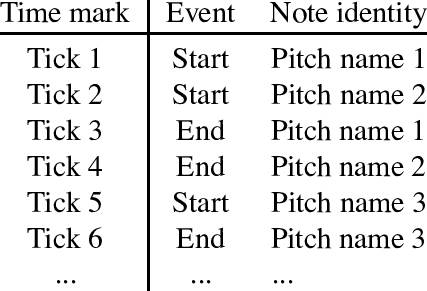
\includegraphics[scale=0.5]{MIDI_file.png}
\centering
\caption{Struktura pliku MIDI. Plik MIDI składa się z tzw. \textit{eventów}, które zawierają informacje o treści wiadomości MIDI oraz o czasie jej nadania. Źródło: \citep[s. 2 - 3]{MIDI_Format} i \citep{Tse2008}.}
\end{figure}

Aby skorzystać z możliwości jakie daje nam MIDI należy zaopatrzyć się w instrumenty. Instrumenty mogą być dystrybuowane niezależnie jako pakiety \textit{VSTi} dołączane oddzielnie do \textit{syntezatora programowego} takiego jak \textit{Helm} (zob. rys. 3.11)
Do tworzenia muzyki w formacie MIDI można wykorzystać także \textit{syntezator sprzętowy} taki jak \textit{klawiatura MIDI}. Klawiatura MIDI jest rodzajem kontrolera wysyłającego sygnały elektryczne w formacie MIDI, które sam protokół interpretuje i odtwarza jako dźwięk. Przykład takiej klawiatury to rysunek 3.12. warto zwrócić uwagę na to, że każdej nucie na klawiaturze przyporządkowany jest odpowiadający mu numer kodu formatu MIDI.

\begin{figure}[H]
\centering
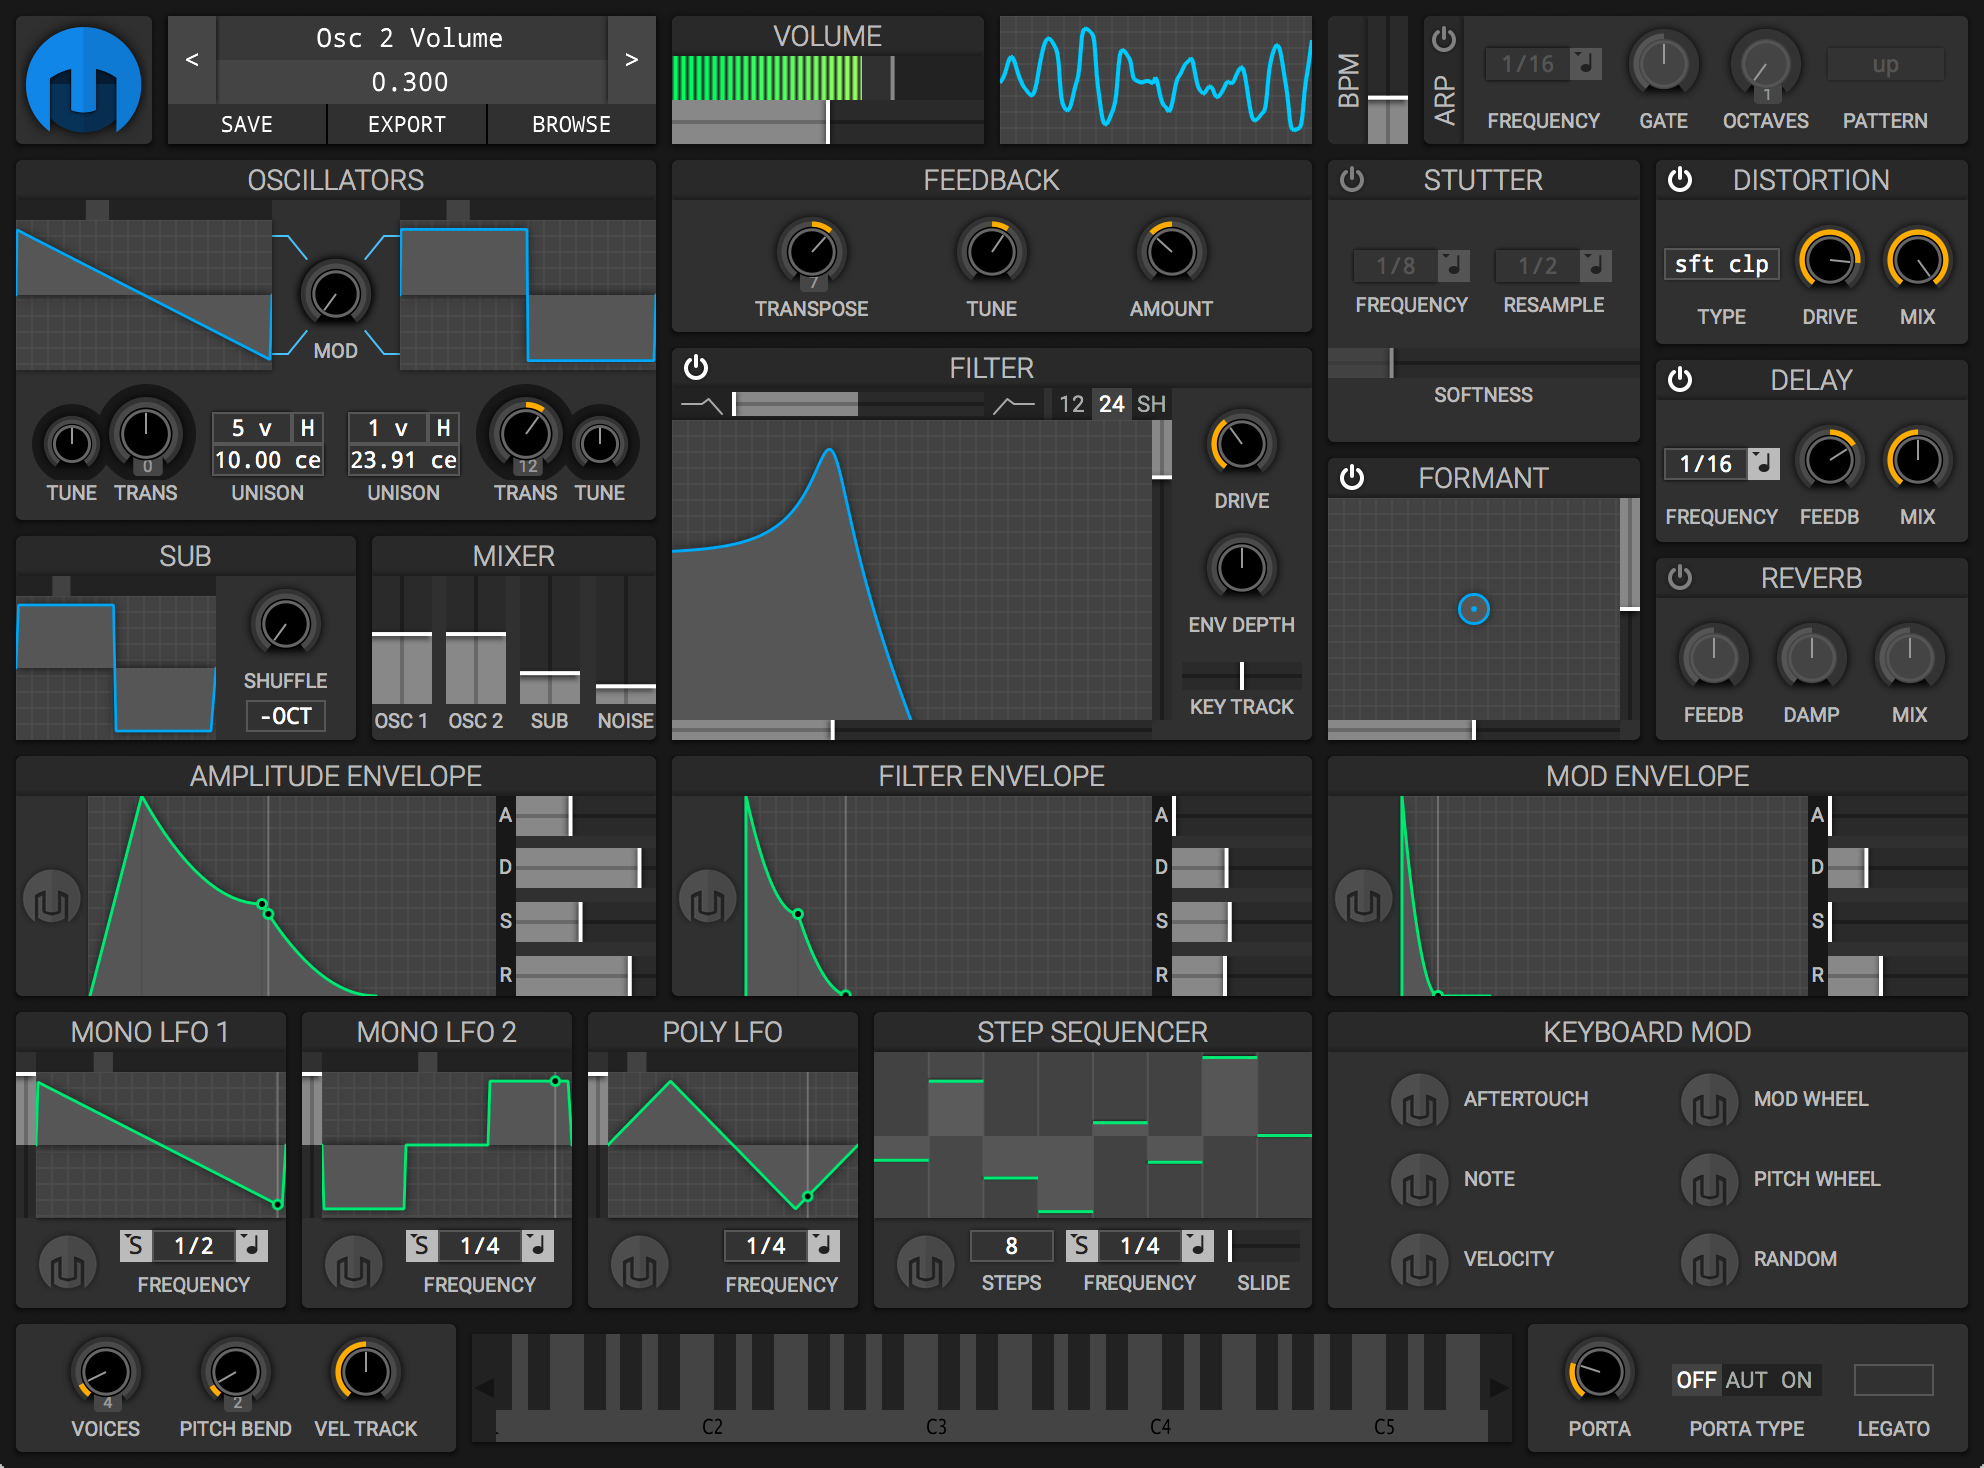
\includegraphics[scale = 0.3]{helm.png}
\centering
\caption{Interfejs programu Helm. Źródło: https://tytel.org/helm/}
\end{figure}


\begin{figure}[H]
\begin{center}
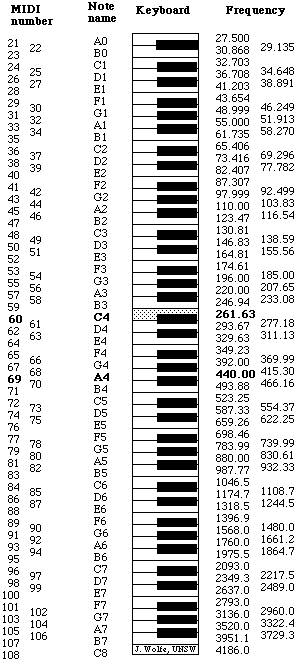
\includegraphics[scale = 0.6]{midi.png}
\centering
\caption{Klawiatura MIDI, Źródło: \href{https://pl.wikipedia.org/wiki/MIDI}{https://pl.wikipedia.org/wiki/MIDI}}
\centering
\end{center}
\end{figure}
 

\chapter{Reprezentacja i klasyfikacja utworu muzycznego}

Na rysunku 18 została przedstawiona gama chromatyczna rozpoczynająca się od dźwięku C:
\begin{figure}[H]
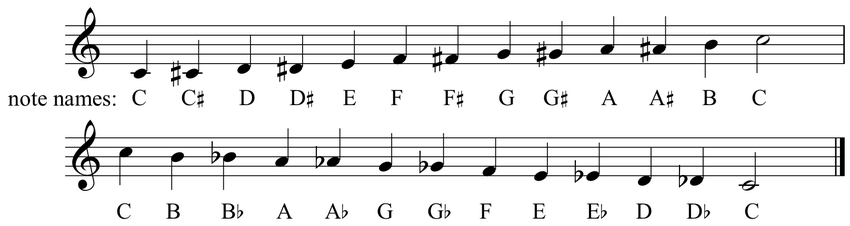
\includegraphics[scale = 0.4]{chromatyczna.png}
\centering
\caption{Skala dwunastodźwiękowa zwana także  \textit{chromatyczną}. Skala chromatyczna to skala, w której poszczególne stopnie oddalone są od siebie o pół tonu. Zawiera wszystkie dźwięki w obrębie danej oktawy, czyli łącznie 12 dźwięków. Krzyżyki oznaczają ruch w górę, bemole ruch w dół. Źródło: \url{https://www.researchgate.net/figure/Chromatic-scale-starting-with-C-22_fig1_334131988}}
\centering
\end{figure}
Skali chromatycznej odpowiada dowolny dwunastowymiarowy wektor wartości formatu \textit{MIDI}. Dla przykładu skala chromatyczna rozpoczynająca się od dźwięku (C, 4), a kończąca się na dźwięku (C, 5), to wektor:
\begin{equation*}
v =
\begin{bmatrix}
60,61,62,63,64,65,66,67,68,69,70,71
\end{bmatrix}
\text{gdzie} \quad v \in \mathbb{R}^{12}.
\end{equation*}

W analogiczny sposób można rozpisać dowolną gamę jako wektor wartości z których każda należy do przestrzeni liczb rzeczywistych. Należy jedynie pamiętać o tym, że wartości liczbowe poszczególnych dźwięków w formacie MIDI różnią się  w zależności of wybranej oktawy i należy je rozpisać zgodnie z powyższą klawiaturą MIDI.



\section{Implementacja zadania klasyfikacji dźwięków}

Stworzona w języku \textit{Haskell} biblioteka \textit{Euterpea}\footnote{https://www.euterpea.com/} pozwala w prosty sposób generować utwory muzyczne. Wykorzystuję się ją szeroko w muzyce algorytmicznej, analizie muzyki i syntezie dźwięku.

\textit{Euterpea} tworzy dźwięki przesyłając komunikaty MIDI do urządzenia, który jest w stanie je odczytać. W najprostszym przypadku takim urządzeniem może być programowy syntezator dźwięku \citep{Obrebski2020}

Prezentowany przeze mnie prosty program w języku Haskell dokonuje klasyfikacji dźwięków, wykorzystując przy tym fragmenty dwóch gotowych utworów muzycznych: 

\begin{enumerate}
    \item Pierwszy utwór \textit{Od Pilicy i Wolbroma} jest przedstawicielem muzyki ludowej i został udostępiony przez Instytut im. Oskara Kolberga (zob. Rysunek 18),
    \item Utwór \textit{Simple Jazz} pobrany z serwisu MuseScore (zob. Rysunek 19).
\end{enumerate}


\begin{figure}[H]
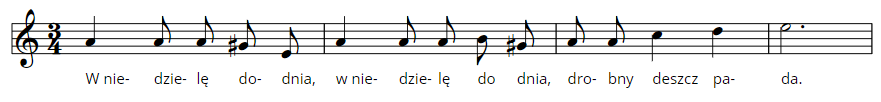
\includegraphics[scale = 0.8]{ludowa.png}
\centering
\caption{Utwór "Od Pilicy i Wolbroma", Źródło: \href{http://oskarkolberg.pl/pl-PL/MusicDb/Details/cafbb535-ed69-4b99-9002-f65fe40ed8fe}{Instytut im. Oskara Kolberga}}
\centering
\end{figure}

Pierwszemu utworowi odpowiada wektor:
\begin{equation*}
    v =
    \begin{bmatrix}
    69,69,69,68,64,69,69,69,71,68,69,69
    \end{bmatrix}
\end{equation*}

\begin{figure}[H]
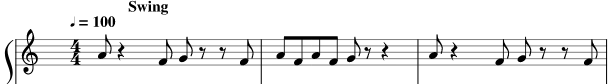
\includegraphics[scale = 0.8]{jazz.png}
\centering
\caption{Fragment utworu "Simple Jazz", Źródło: \href{https://musescore.com/user/27009977/scores/5429135}{Musescore.com}}
\centering
\end{figure}
Drugiemu utworowi odpowiada wektor $u$:
\begin{equation*}
u =
    \begin{bmatrix}
    69,65,67,65,69,65,69,65,67,71,65,67
    \end{bmatrix}
\end{equation*}

Funkcje dokonujące obliczeń zostały zadeklarowane w następujący sposób:
\begin{lstlisting}[language = Haskell]
-- odejmowanie dwoch wektorow
odejmij :: [Float] -> [Float] -> [Float]
odejmij [] _ = []
odejmij _ [] = []
odejmij (x:xs) (y:ys) = x - y : (odejmij xs ys)


-- Iloczyn skalarny
dot :: [Float] -> [Float] -> Float
dot x y = sum $ zipWith (*) x y

klasyfikacja:: Float -> Int
klasyfikacja y_x
    | y_x > w_0 = 1 -- klasa C1
    | y_x < w_0 = -1 --klasa C2

toAbsPitches :: [Pitch] -> [AbsPitch]
toAbsPitches ps = map absPitch ps


toPitches :: [AbsPitch] -> [Pitch]
toPitches as = map pitch as
\end{lstlisting}

Pomocnicze funkcje \textit{ToPitches} i \textit{toAbsPitches} umożliwiają konwersje z  zapisu nutowego do liczb całkowitych i odwrotnie \citep[s. 60]{HSOM_2018}.

Klasyfikacje możemy przeprowadzić na dwa sposoby:
\begin{itemize}
    \item Na podstawie podobieństwa poszczególnych dźwięków do siebie,
    \item Na podstawie mierzalnych cech, które opisują utwór muzyczny. W tym wypadku skupimy się na \textit{rytmie}.
\end{itemize}

\subsection{4.2 Klasyfikacja na podstawie podobieństwa dźwięków}
Mając dane dwa wektory $v$ i $u$, sprawdźmy, czy wektor $x$ jest bardziej podobny do muzyki ludowej ($C_{1}$), reprezentowanej przez wektor $v$, czy do muzyki jazzowej ($C_{2}$), reprezentowanej przez $u$. 

\begin{equation*}
v =
\begin{bmatrix}
69,69,69,68,64,69,69,69,71,68,69,69
\end{bmatrix}
\end{equation*}

\begin{equation*}
    u =
    \begin{bmatrix}
    69,65,67,65,69,65,69,65,67,71,65,67
    \end{bmatrix}
\end{equation*}

Jako pierwszy przykład testowy wykorzystamy fragment utworu \textit{The Entertainer} (zob.rys. 21) który zakodowaliśmy jako wektor $x$:
\begin{equation*}
x =
    \begin{bmatrix}
   60,60,60,60,60,60,62,63,60,62,64,64
    \end{bmatrix}
\end{equation*}

\begin{figure}[H]
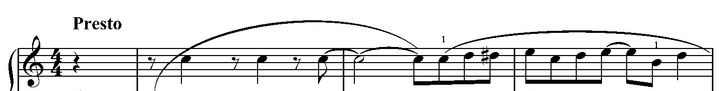
\includegraphics[scale = 0.7]{entertainer.png}
\centering
\caption{Fragment utworu "The Entertainer". Źródło: \url{https://www.8notes.com/scores/13178.asp}}
\centering
\end{figure}

Przebieg klasyfikacji przebiega następująco. Najpierw obliczamy $y$:
\begin{align*}
y = [(69 - 69), (69 - 65), (69 - 67), (68 - 65), \\ (64 - 69), 
(69 - 65), (69 - 69), (69 - 65),\\ (71 - 67), (68 - 71), (69 - 65), (69 - 67)].
\end{align*}

Zatem:
\begin{equation*}
y =  [0, 4, 2, 3, -5, 4, 0, 4, 4, -3, 4, 2].
\end{equation*}

Następnie obliczamy $w_{0}$:
\begin{align*}
w_{0} = &  \frac{1}{2} \big(\|v\|^{2} - \|u\|^{2}\big)  \\
= & \frac{1}{2}[(69 \cdot 69) + (69 \cdot 69) + (69 \cdot 69) + (68 \cdot 68) \\
 & + (64 \cdot 64) + (69 \cdot 69) + (69 \cdot 69) + (69 \cdot 69) \\
 & + (71 \cdot 71) + (68 \cdot 68)  + (69 \cdot 69) + (69 \cdot 69) \\
 - & (69 \cdot 69) + (65 \cdot 65) + (67 \cdot 67) + (65 \cdot 65) \\
 & + (69 \cdot 69) + (65 \cdot 65) + (69 \cdot 69) + (65 \cdot 65) \\
 & + (67 \cdot 67) + (71 \cdot 71) + (65 \cdot 65) + (67 \cdot 67)] \\
 = & \frac{1}{2}(56473 - 53916) \\
 = & \frac{1}{2}(2557) = 1278,5.
\end{align*}
Wtedy:
\begin{align*}
\big \langle y|x  \big \rangle  = \quad 
& [0, 4, 2, 3, -5, 4, 0, 4, 4, -3, 4, 2] \\ 
&\cdot
[60,60,60,60,60,60,62,63,60,62,64,64] 
= 1170.
\end{align*}
Jeśli, $\big \langle y|x \big \rangle < w_{0}$, to $f(x) = -1$, a to oznacza przydział do klasy $C_{2}$.

Klasyfikator uznał zatem, że dźwięki w wektorze $x$ są bardziej podobne do tych w wektorze $u$. Bluesowy utwór \textit{The Entertainer} został uznany za bardziej podobny do jazzu niż do muzyki ludowej, co raczej zgadza się z powszechną intuicją Ten sposób klasyfikacji nie jest optymalny, ponieważ pomija wszystkie inne cechy utworu, takie jak \textit{rytm}. W kolejnym podrozdziale pokażemy jak można rozwiązać ten problem i zamodelujemy klasyfikacje na podstawie rytmu.

\section{Modelowanie binarne typu cisza - dźwięk}

Sposobem na klasyfikacje utworów względem ich rytmu jest takie zamodelowanie wektora wejściowego nut, gdzie do każdej wartości dźwiękowej, (nie będącej pauzą), przyporządkowujemy wartość 1, a każdej wartości będącej pauzą przyporządkowujemy wartość 0. Przyporządkowanie to zawsze działa w taki sam sposób, niezależnie od tego jakiej długości jest dana nuta, czy pauza. Prosty przykład jak miałoby to wyglądać został przedstawiony na rys. 20.

\begin{figure}[H]
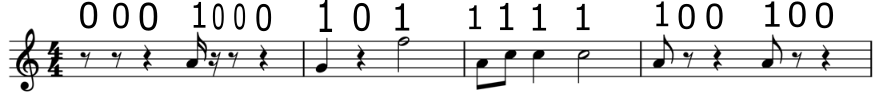
\includegraphics[scale = 0.5]{test.png}
\centering
\caption{Przykład binarnego modelowania na pięciolinii. Wartość "1" przyporządkowujemy jedynie dźwiękom, niezależnie od długości i trwania, a wartość "0" zostawiamy dla pauz. Źródło: Opracowanie własne w programie \textit{MuseScore} i \textit{Inkscape}.}
\centering
\end{figure}

Powiedzieliśmy sobie wcześniej, że rytm jest zmienną odpowiedzialną za czasową organizacje przebiegu utworu. Zbudowanie wektora nut w taki sposób da nam możliwość śledzenia ile występuje pauz i dźwięków i w jakiej one są kolejności, a dzięki temu będziemy mieli możliwość porównywania utworów pod względem ich struktury. Takie rozwiązanie sprawia, że uzyskujemy więcej informacji o melodii, niż miało to miejsce w przypadku porównywania samych dźwięków, bez uwzględniania ich kolejności.
Wykorzystamy tym razem próbkę złożoną z 21 wartości dźwięków i pauz, żeby badane wektory $v$, $u$ oraz $x$ zgadzały się ze sobą pod względem wymiarów.

Na początku ustalmy wektory $v$, $u$ oraz $x$
\begin{equation*}
    v = 
    \begin{bmatrix}
    1,0,1,1,1,1,1,0,1,1,1,1,1,1,1,1,1,0,1,1,1
    \end{bmatrix}
\end{equation*}

\begin{equation*}
    u =
    \begin{bmatrix}
    1,0,1,1,0,0,1,1,1,1,1,1,0,0,1,0,1,1,0,0,1
    \end{bmatrix}
\end{equation*}

\begin{equation*}
    x =
    \begin{bmatrix}
    0,1,0,1,0,1,1,1,1,1,1,1,1,1,1,1,1,1,1,1,1
    \end{bmatrix}
\end{equation*}

Na tej podstawie dokonujemy klasyfikacji.
Zatem:
\begin{equation*}
    y = v - u =
    \begin{bmatrix}
    0,0,0,0,1,1,0,-1,0,0,0,0,1,1,0,1,0,-1,1,1,0
    \end{bmatrix}
\end{equation*}
Następnie:

\begin{equation*}
w_{0} =\frac{1}{2} \big(\|v\|^{2} - \|u\|^{2}\big) = 2.5.
\end{equation*}
Wtedy:
\begin{equation*}
\big \langle y|x  \big \rangle = 2.0.
\end{equation*}
Stąd:
\begin{equation*}
    \big \langle y|x \big \rangle < w_{0}, \quad \text{wtedy} \quad f(x) = -1
\end{equation*}
A to również oznacza przydział do klasy $C_{2}$.
Zatem klasyfikując na podstawie rytmu program ponownie uznał, że bluesowy utwór \textit{The Entertainer} brzmi bardziej jazzowo niż ludowo.

\subsection{4.4 Procedura testowa}
Na podstawie powyżej opisanych dwóch metod przeprowadzono testy dla większej ilości utworów. Przebieg procedury testowania był następujący:
\begin{enumerate}
    \item Wygenerowanie losowego wektora $x$,
    \item Obliczenie $y = v - u$,
    \item Obliczenie wartości $w_{0} =\frac{1}{2} \big(\|v\|^{2} - \|u\|^{2}\big)$,
    \item Obliczenie $\big \langle y|x \big \rangle$,
    \item Przydział wektora $x$ do klasy $C_{1}$ lub $C_{2}$.
\end{enumerate}

Jako, że wzorcowe wektory $v$ i $u$ zostały wprowadzone jako wartości całkowite, a do obliczenia iloczynu skalarnego potrzebujemy listy wartości zmiennoprzecinkowych, to ich konwersja na typ \textit{Float} została przeprowadzona przy pomocy funkcji \textit{floatList} zaimplementowanej następująco

\begin{lstlisting}[language = Haskell]

-- Konwersja listy int na float
floatList :: [AbsPitch] -> [Float]
floatList [] = []
floatList (n:ns)  = (x) : floatList(ns)
    where x = fromIntegral n :: Float 
\end{lstlisting}

Testy przeprowadzono w dwóch wariantach. W wariancie pierwszym (A) porównywano wektor wzorcowy danego typu muzyki (ludowej bądź jazzowej), z innym utworem z tego samego gatunku muzyki. Przykłady zostały pobrane z seriwsu \textit{MuseScore} lub z \textit{Instytutu im. Oskara Kolberga}, odpowiednio 5 utworów muzyki ludowej lub jazzowej. W wariancie (B) wektory wzorcowe były porównywane z losowo wygenerowanym innym wektorem, żeby sprawdzić jakie decyzje podejmuje algorytm dla losowo wygenerowanych sekwencji dźwięków. 

\subsection{(A) Porównywanie utworu wzorcowego z innym utworem}
\FloatBarrier
\begin{table}[h]
\centering
\begin{tabular}{|c|c|c|}
\hline
Lp. & $X_{input}$ & $X_{output}$ \\ \hline
1.   & $C_{1}$      & $C_{2}$      \\ \hline
2.   & $C_{1}$      & $C_{1}$     \\ \hline
3.   & $C_{1}$      & $C_{2}$      \\ \hline
4.   & $C_{1}$      & $C_{1}$     \\ \hline
5.   & $C_{1}$      & $C_{1}$      \\ \hline
6.   & $C_{2}$      & $C_{2}$    \\ \hline
7.   & $C_{2}$      & $C_{2}$     \\ \hline
8.   & $C_{2}$      & $C_{2}$     \\ \hline
9.   & $C_{2}$      & $C_{1}$     \\ \hline
10.  & $C_{2}$      & $C_{2}$      \\ \hline
\end{tabular}
\caption{Wyniki klasyfikacji na podstawie podobieństwa dźwięków. Źródło: Opracowanie własne.}
\end{table}
\FloatBarrier

\textbf{Podsumowanie:}
Wyniki klasyfikacji na podstawie podobieństwa dźwięków kształtują się następująco:

\begin{enumerate}
    \item Dla muzyki ludowej klasyfikator osiągnął 60\% dokładności (2 z 5 utworów zaklasyfikowano źle)
    \item Dla muzyki jazzowej klasyfikator osiągnął 80\% dokładności (1 z 5 utworów zaklasyfikowano źle)
\end{enumerate}

\textbf{Łącznie dla 10 przypadków, 7 razy dokonano poprawnej klasyfikacji (70\% dokładności)}.
\FloatBarrier
\begin{table}[h]
\begin{tabular}{|c|c|c|}
\hline
Lp. & $X_{input}$ & $X_{output}$ \\ \hline
1.   & $C_{1}$      & $C_{1}$      \\ \hline
2.   & $C_{1}$      & $C_{1}$     \\ \hline
3.   & $C_{1}$      & $C_{1}$      \\ \hline
4.   & $C_{1}$      & $C_{1}$     \\ \hline
5.   & $C_{1}$      & $C_{1}$      \\ \hline
6.   & $C_{2}$      & $C_{2}$    \\ \hline
7.   & $C_{2}$      & $C_{2}$     \\ \hline
8.   & $C_{2}$      & $C_{1}$     \\ \hline
9.   & $C_{2}$      & $C_{2}$     \\ \hline
10.  & $C_{2}$      & $C_{2}$      \\ \hline
\end{tabular}
\centering
\caption{Wyniki klasyfikacji na podstawie podobieństwa rytmu. Źródło: Opracowanie własne.}
\end{table}
\FloatBarrier

\textbf{Podsumowanie:}
Wyniki klasyfikacji na podstawie podobieństwa rytmu kształtują się następująco:

\begin{enumerate}
    \item Dla muzyki ludowej klasyfikator osiągnął 100\% dokładności (0 z 5 utworów zaklasyfikowano źle)
    \item Dla muzyki jazzowej klasyfikator osiągnął 90\% dokładności (1 z 5 utworów zaklasyfikowano źle)
\end{enumerate}

\textbf{Łącznie dla 10 przypadków, 9 razy dokonano poprawnej klasyfikacji (90\% dokładności)}.





\subsection{(B) Porównywanie utworu wzorcowego z utworem losowym}

Generowanie losowego wektora nut przeprowadzono za pomocą monady zaimplementowanej w następujący sposób:
\begin{lstlisting}[language = Haskell]

import System.Random (randomRIO) 
-- funkcje generujace listy 
randomFloat :: Float -> IO([Float])
randomFloat 0 = return []
randomFloat n = do
  r  <- randomRIO (20, 108) -- zakres
  rs <- randomFloat (n-1) -- generuje liste
  return (r:rs)
  
randomBin :: Int -> IO([Int])
randomBin 0 = return []
randomBin n = do
    r <- randomRIO (1,0) -- zakres
    rs <- randomBin (n-1)
    return (r:rs)
\end{lstlisting}

Funkcja \textit{randomFloat} generuje wektor wartości dźwiękowych o dowolnej długości, zakres losowania zmieniał się co iteracje i został ustalony na przedział 20 - 108, co odpowiada zakresowi wartości formatu \textit{MIDI}. Funkcja \textit{randomBin} generuje wektor złożony z zer i jedynek, również o dowolnej długości.
\FloatBarrier
\begin{table}[h]
\begin{tabular}{|c|c|c|}
\hline
Lp. & $X_{input}$ & $X_{output}$ \\ \hline
1.   & $C_{1}$      & $C_{1}$      \\ \hline
2.   & $C_{1}$      & $C_{2}$     \\ \hline
3.   & $C_{1}$      & $C_{1}$      \\ \hline
4.   & $C_{1}$      & $C_{1}$     \\ \hline
5.   & $C_{1}$      & $C_{1}$      \\ \hline
6.   & $C_{2}$      & $C_{1}$    \\ \hline
7.   & $C_{2}$      & $C_{2}$     \\ \hline
8.   & $C_{2}$      & $C_{2}$     \\ \hline
9.   & $C_{2}$      & $C_{2}$     \\ \hline
10.  & $C_{2}$      & $C_{1}$      \\ \hline
\end{tabular}
\centering
\caption{Wyniki klasyfikacji na podstawie podobieństwa dźwięków dla wektorów losowych. Źródło: Opracowanie własne.}
\end{table}
\FloatBarrier

\textbf{Podsumowanie:}
Wyniki klasyfikacji na podstawie podobieństwa rytmu kształtują się następująco:

\begin{enumerate}
    \item Dla muzyki ludowej klasyfikator osiągnął 80\% dokładności (1 z 5 utworów zaklasyfikowano źle)
    \item Dla muzyki jazzowej klasyfikator osiągnął 60\% dokładności (2 z 5 utworów zaklasyfikowano źle)
\end{enumerate}

\textbf{Łącznie dla 10 przypadków, 7 razy dokonano poprawnej klasyfikacji (70\% dokładności)}.
\FloatBarrier
\begin{table}[h]
\begin{tabular}{|c|c|c|}
\hline
Lp. & $X_{input}$ & $X_{output}$ \\ \hline
1.   & $C_{1}$      & $C_{1}$      \\ \hline
2.   & $C_{1}$      & $C_{2}$     \\ \hline
3.   & $C_{1}$      & $C_{2}$      \\ \hline
4.   & $C_{1}$      & $C_{2}$     \\ \hline
5.   & $C_{1}$      & $C_{2}$      \\ \hline
6.   & $C_{2}$      & $C_{2}$    \\ \hline
7.   & $C_{2}$      & $C_{2}$     \\ \hline
8.   & $C_{2}$      & $C_{1}$     \\ \hline
9.   & $C_{2}$      & $C_{1}$     \\ \hline
10.  & $C_{2}$      & $C_{2}$      \\ \hline
\end{tabular}
\centering
\caption{Wyniki klasyfikacji na podstawie podobieństwa rytmu dla wektorów losowych. Źródło: Opracowanie własne.}
\end{table}
\FloatBarrier

\textbf{Podsumowanie:}
Wyniki klasyfikacji na podstawie podobieństwa rytmu kształtują się następująco:

\begin{enumerate}
    \item Dla muzyki ludowej klasyfikator osiągnął 10\% dokładności (4 z 5 utworów zaklasyfikowano źle)
    \item Dla muzyki jazzowej klasyfikator osiągnął 40\% dokładności (3 z 5 utworów zaklasyfikowano źle)
\end{enumerate}

\textbf{Łącznie dla 10 przypadków, 3 razy dokonano poprawnej klasyfikacji (30\% dokładności)}.

\section{Wnioski}

Najlepsze wyniki klasyfikacji osiągnięto podczas testowania na utworach rzeczywistych. Algorytm osiągał porównywalnie gorsze wyniki w wariancie z utworami generowanymi losowo. Klasyfikacja na podstawie podobieństwa dźwięków osiągała gorsze wyniki niż klasyfikacja na podstawie rytmu dla utworów rzeczywistych, ale jej skuteczność znacznie się pogorszyła dla utworów generowanych losowo, co może oznaczać, że algorytm klasyfikacji faktycznie dobrze wykrywa rytm melodii. Głównym wnioskiem płynącym z badań jest teza, że klasyfikacja na podstawie rytmu jest dokładniejsza, ale żeby ją potwierdzić, bądź odrzucić należało by wykonać testy dla większej ilości przypadków testowych.

\chapter{Przekształcenia geometryczne w przestrzeni}

\textit{Przekształceniem geometrycznym} lub \textit{odwzorowaniem geometrycznym} nazywamy funkcję, której dziedziną i przeciwdziedziną jest zbiór wszystkich punktów przestrzeni $\mathbb{R}^{n}$. W węższym znaczeniu jest to funkcja wzajemnie jednoznaczna przekształcająca jeden zbiór punktów, zwany \textit{figurą geometryczną} lub \textit{wektorem} w inny obiekt tego samego typu.\footnote{Źródło: https://www.math.edu.pl/przeksztalcenia-w-przestrzeni [Dostęp: 26.01.22]} 

\section{Definicja macierzy}
Układ $m \cdot n$ elementów $a_{ij} \in \mathbb{R}$ $(i = 1,\cdots,m, j = 1,\cdots,n)$ zapisany w następującej postaci:
\begin{equation*}
    \begin{bmatrix}
    a_{11} & \cdots & a_{1n} \\
    \cdots & \cdots & \cdots \\
    a_{m1} & \cdots & a_{mn}
    \end{bmatrix}
\end{equation*}
nazywamy macierzą o $m$ wierszach i $n$ kolumnach zdefiniowaną nad ciałem $\mathbb{R}$ (lub macierzą wymiaru $m \times n$). \citep[s. 85]{Repetytorium1977}.
Macierz można też zapisywać krócej:
\begin{equation*}
\mathbb{A} = [a_{i,j}]_{m\times n}    
\end{equation*}

Liczby zawarte w macierzy nazywamy jej \textit{elementami} (zob. rys. 23) \citep[s. 18]{Rutkowski_2008}.

\begin{figure}[H]
\begin{equation*}
\mathbb{A} =
    \begin{bmatrix}
    1 & 2 \\
    3 & 4 \\
    1 & 0
    \end{bmatrix}
\end{equation*}
\centering
\caption{Macierz prostokątna $\mathbb{A }$ wymiaru $3 \times 2$.}
\end{figure}

Macierz o wymiarach $n \times n$ nazywamy \textit{macierzą kwadratową stopnia n} (zob. rys. 24).

\begin{figure}[H]
\begin{equation*}
\mathbb{B} =
    \begin{bmatrix}
    1 & 2 & 3 & 4 \\
    5 & 6 & 7 & 8 \\
    9 & 10 & 11 & 12 \\
    13 & 14 & 15 & 16
    \end{bmatrix}
\end{equation*}
\centering
\caption{Macierz kwadratowa $\mathbb{B}$ wymiaru $4 \times 4$. Macierz kwadratowa ma taką samą liczbę wierszy i kolumn.}
\end{figure}

Odwołanie się do elementu macierzy następuje poprzez nazwę macierzy wraz z towarzyszącym jej dolnym indeksem wierszowym i kolumnowym. Dla przykładowej macierzy $\mathbb{A}_{3\times3}$ indeksy elementów wyglądają następująco:

\begin{equation*}
\mathbb{A}_{3\times3} =
    \begin{bmatrix}
    \mathbf{a_{11}} & a_{12} & a_{13} \\
    a_{21} & \mathbf{a_{22}} & a_{23} \\
    a_{31} & a_{32} & \mathbf{a_{33}}
    \end{bmatrix}
\end{equation*}
Pogrubieniem oznaczono tak zwaną \textit{przekątną główną macierzy}, którą tworzą elementy o równych wartościach indeksów wierszowych i kolumnowych.

\textit{Wektorem wierszowym} nazywamy macierz złożoną tylko z jednego wiersza. Na przykład:

\begin{equation*}
    \mathbb{A}_{1\times3} =
    \begin{bmatrix}
   1 & 2 & 3
    \end{bmatrix}
\end{equation*}

Analogicznie, \textit{wektorem kolumnowym} nazywamy macierz złożoną tylko  z pojedynczej kolumny:
\begin{equation*}
    \mathbb{A}_{3\times1} =
    \begin{bmatrix}
    1 \\ 2 \\ 3
    \end{bmatrix}
\end{equation*}

\section{Iloczyn macierzy}
\begin{definicja}
Iloczynem macierzy\footnote{Opracowano na podstawie \citep[s. 88]{Repetytorium1977}}
\begin{equation*}
\begin{bmatrix}
a_{11} & \cdots & a_{1n} \\
\vdots \\
a_{m1} & \cdots & a_{mn}
\end{bmatrix}
\in \mathbb{M}_{m \times n} \quad ,
\begin{bmatrix}
b_{11} & \cdots & b_{1p} \\
\vdots \\
b_{n1} & \cdots & b_{np}
\end{bmatrix}
\in \mathbb{M}_{n \times p} 
\end{equation*}
nazywamy macierz
\begin{equation*}
\begin{bmatrix}
c_{11} & \cdots & c_{1p} \\
\vdots \\
c_{m1} & \cdots & c_{mp}
\end{bmatrix}
\in \mathbb{M}_{m \times p} \, ,
\end{equation*}
gdzie 
\begin{equation*}
    c_{ij} = \sum^{n}_{k=1} a_{ik} b_{kj}
\end{equation*}
i piszemy
\begin{equation*}
    [c_{ij}] = [a_{ij}] \cdot [b_{ij}] \ \text{lub} \ [a_{ij}][b_{ij}].
\end{equation*}
\end{definicja}
\begin{przyklad}

Załóżmy, że mamy dwie macierze, macierz $\mathbb{A}_{2 \times 3}$ i macierz $\mathbb{B}_{3\times 2}$. Po ich pomnożeniu otrzymamy nową macierz $\mathbb{C}$, która posiada tyle wierszy ile miała macierz $\mathbb{A}$ i tyle kolumn ile miała macierz $\mathbb{B}$. Zatem w tym wypadku macierz $\mathbb{C}$ ma 2 wiersze i 2 kolumny. 
Zatem mnożenie:
\begin{equation*}
    \mathbb{A}_{2 \times 3} =
    \begin{bmatrix}
    1 & 2 & 3 \\
    4 & 5 & 6
    \end{bmatrix}
    ,\quad  
    \mathbb{B}_{3 \times 2} =
    \begin{bmatrix}
    1 & 3 \\
    2 & 4 \\
    1 & 2
    \end{bmatrix}
\end{equation*}
daje nam:
\begin{equation*}
    \mathbb{C}_{2\times 2} =
    \begin{bmatrix}
    1 \cdot 1 + 2 \cdot 2 + 3 \cdot 1 & 1 \cdot 3 + 2 \cdot 4 + 3 \cdot 2 \\
    4 \cdot 1 + 5 \cdot 2 + 6 \cdot 1 & 4 \cdot 3 + 5 \cdot 4 + 6 \cdot 2
    \end{bmatrix}
    =
    \begin{bmatrix}
    8 & 17 \\
    20 & 44
    \end{bmatrix}
\end{equation*}.
\end{przyklad}

Jak można zauważyć macierz $\mathbb{C}$ jest sumą iloczynów kolejnych elementów z każdego wiersza macierzy $\mathbb{A}$ przez każdy kolejny element z każdej kolumny macierzy $\mathbb{B}$.
Operacja mnożenia macierzy jest przydatna do wyznaczenia tzw. \textit{Macierzy obrotu}.




\subsection{Macierz obrotu}
Macierz obrotu to szczególny rodzaj macierzy, umożliwiający poprzez mnożenie z  danym wektorem $v$ wymiaru $n$ uzyskanie nowego wektora $v'$ obróconego o zadany kąt $\phi$ względem początku układu współrzędnych umieszczonego nad ciałem $\mathbb{R}^{n}$.\footnote{Źródło: \url{https://www.obliczeniowo.com.pl/258}}

\section{Obroty w \texorpdfstring{$\mathbb{R}^{2}$}{Obroty w R2}}

\begin{figure}[H]
    \centering
    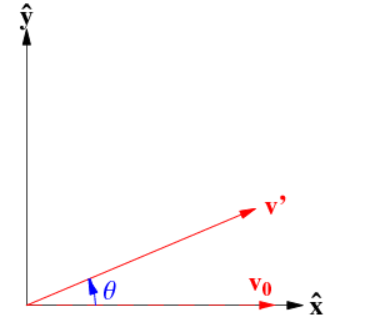
\includegraphics[scale=0.8]{RotationMatrix.png}
    \caption{ Obrót wektora $v_{0}$ o kąt $\phi$ względem osi $x$. Za: \citep{Weisstein2000}.}
\end{figure}

Macierz obrotu w $\mathbb{R}^{2}$ oznaczamy zwykle symbolem $R(\phi)$\footnote{Za: \citep{Weisstein2000}.}:

\begin{equation*}
R(\phi) =
    \begin{bmatrix}
    \cos\phi & -\sin\phi \\
    \sin\phi & \cos\phi
    \end{bmatrix}
\end{equation*}
Zatem:
\begin{equation*}
    v' = R_{\phi} \cdot v_{0}.
\end{equation*}
Obrót wektora w $\mathbb{R}^{2}$ można wtedy wykonać poprzez zwykłe mnożenie macierzowe w następujący sposób:

\begin{equation*}
    v = R(\phi) \cdot v =
    \begin{bmatrix}
    \cos\phi & -\sin\phi \\
    \sin\phi & \cos\phi 
    \end{bmatrix}
    \cdot
    \begin{bmatrix}
    x \\
    y
    \end{bmatrix}
    =
    \begin{bmatrix}
    x \cdot \cos\phi & - & y \cdot \sin\phi \\
    x \cdot \sin\phi & + & y \cdot \cos\phi
    \end{bmatrix}
\end{equation*}
Macierz ta obraca wektory kolumnowe w następujący sposób:

\begin{equation*}
v' =
    \begin{bmatrix}
    x' \\
    y
    \end{bmatrix}
    =
    \begin{bmatrix}
    \cos\phi & -\sin\phi \\
    \sin\phi & \cos\phi
    \end{bmatrix}
    \cdot
    \begin{bmatrix}
    x \\
    y
    \end{bmatrix}
\end{equation*}
Wtedy współrzędne wektora:  
\begin{equation*}
v' =
    \begin{bmatrix}
     x' \\
     y'
    \end{bmatrix}
\end{equation*}
mają wartości:
\begin{equation*}
    x' = x \cos\phi - y \sin\phi
\end{equation*},
\begin{equation*}
    y' = x \sin\phi + y \cos\phi
\end{equation*}.

Obrót jest przeciwny do obrotu zgodnego z ruchem wskazówek zegara jeżeli kąt $\phi$ jest dodatni. Macierz obrotu zgodnego z ruchem wskazówek zegara ma postać:

\begin{equation*}
    R(-\phi) =
    \begin{bmatrix}
    \cos\phi & \sin\phi \\
    -\sin\phi & \cos\phi
    \end{bmatrix}
\end{equation*}

Obroty w $\mathbb{R}^{2}$ spełniają własność przemienności. To znaczy, że nie ma znaczenia kolejność wykonywania obrotów. Niezależnie od kolejności otrzymuje się takie same wartości w wektorze wynikowym.
Załóżmy, że mamy wektor:
\begin{equation*}
v =
    \begin{bmatrix}
    1 \\
    0
    \end{bmatrix}
\end{equation*}
\begin{przyklad}
Obróćmy wektor $v$ o kąt $45^{\circ}$ w kierunku zgodnym i przeciwnym do ruchu wskazówek zegara:
\begin{equation*}
    R(45^{\circ}) =
    \begin{bmatrix}
    1 \\
    0
    \end{bmatrix}
    \cdot
    \begin{bmatrix}
    \cos\phi & -\sin\phi \\
    \sin\phi & \cos\phi
    \end{bmatrix}
\end{equation*}
Z tego wynika, że współrzędne wynoszą:
\begin{equation*}
    x' = 1 \cdot \frac{\sqrt{2}}{2} - 0 \cdot \frac{\sqrt{2}}{2}
    = \frac{1}{\sqrt{2}}
\end{equation*}
oraz
\begin{equation*}
    y' = 1 \cdot \frac{\sqrt{2}}{2} + 0 \cdot \frac{\sqrt{2}}{2} = \frac{1}{\sqrt{2}}
\end{equation*}
Zatem otrzymane współrzędne wektora $v'$ przy obrocie w kierunku przeciwnym do ruchu wskazówek zegara wynoszą:
\begin{equation*}
v' =
    \begin{bmatrix}
    \frac{1}{\sqrt{2}} \\
    \frac{1}{\sqrt{2}}
    \end{bmatrix}
\end{equation*}

\begin{equation*}
    R(-45^{\circ}) =
    \begin{bmatrix}
    1 \\
    0
    \end{bmatrix}
    \cdot
    \begin{bmatrix}
    \cos\phi & \sin\phi \\
    -\sin\phi & \cos\phi
    \end{bmatrix}
\end{equation*}
Zatem współrzędne $x'$ i $y'$ wynoszą:
\begin{equation*}
 x' = 1 \cdot -(\frac{\sqrt{2}}{2}) - 0 \cdot -(\frac{\sqrt{2}}{2})
     = -(\frac{1}{\sqrt{2}})
\end{equation*}
\begin{equation*}
     y' = 1 \cdot -(\frac{\sqrt{2}}{2}) + 0 \cdot -(\frac{\sqrt{2}}{2})
     = -(\frac{1}{\sqrt{2}})
\end{equation*}
Otrzymujemy zatem, że współrzędne wektora $v'$ dla obrotu w kierunku zgodnym z kierunkiem ruchu wskazówek zegara wynoszą: 
\begin{equation*}
v' =
    \begin{bmatrix}
    -\frac{1}{\sqrt{2}} \\
    -\frac{1}{\sqrt{2}}
    \end{bmatrix}
\end{equation*}
\end{przyklad}
\section{Obroty w \texorpdfstring{$\mathbb{R}^{3}$}{Obroty w R3} }
Poniżej definiujemy macierze elementarne, które obracają wektor $v$ względem, kolejno: osi $Ox$, $Oy$ oraz $Oz$. Macierze obrotu mają postać:
\begin{equation*}
R_{x}(\phi) =
    \begin{bmatrix}
    1 & 0 & 0 \\
    0 & \cos\phi & -\sin\phi \\
    0 & \sin\phi & \cos\phi 
    \end{bmatrix}
    \end{equation*}
    \\
    \begin{equation*}
    R_{y}(\phi) =
    \begin{bmatrix}
    \cos\phi & 0 & \sin\phi \\
    0 & 1 & 0  \\
    -\sin\phi & 0 & \cos\phi
    \end{bmatrix}
    \end{equation*}
    \\
    \begin{equation*}
        R_{z}(\phi) =
        \begin{bmatrix}
        \cos\phi & -\sin\phi & 0 \\
        \sin\phi & \cos\phi & 0 \\
        0 & 0 & 1
        \end{bmatrix}
    \end{equation*}

\begin{przyklad}
    
Macierz $R_{z}(\phi)$ dla kąta $\phi = 90^{\circ}$ obraca wektor $v$ względem osi $OZ$. Współrzędne wektora $v'$ można wyliczyć dokonując pomnożenia macierzy $R_{z}$ przez wektor $v$ postaci:
\begin{equation*}
v = 
    \begin{bmatrix}
    1 \\
    0 \\
    0
    \end{bmatrix}
\end{equation*}

\begin{equation*}
 R_{z}(90^{\circ}) = 
\begin{bmatrix}
    1 \\
    0 \\ 
    0
    \end{bmatrix}
    \cdot
    \begin{bmatrix}
\cos90^{\circ} & -\sin 90^{\circ} &  0 \\
\sin 90^{\circ} & \cos 90^{\circ} &  0 \\
0 & 0 & 1
    \end{bmatrix}
    = 
    \begin{bmatrix}
    0 & -1 & 0 \\
    1 & 0 & 0 \\
    0 & 0 & 1
    \end{bmatrix}
    \cdot
    \begin{bmatrix}
    1 \\
    0 \\
    0
    \end{bmatrix}
    =
    \begin{bmatrix}
    0 \\
    1 \\
    0
    \end{bmatrix}
\end{equation*}
Analogiczne obliczenia możemy wykonać także dla pozostałych osi.
Oś $OX$:

\begin{equation*}
 R_{x}(90^{\circ}) = 
\begin{bmatrix}
    1 \\
    0 \\ 
    0
    \end{bmatrix}
    \cdot
    \begin{bmatrix}
     1 & 0 & 0 \\
    0 & \cos 90^{\circ} & -\sin90^{\circ} \\
    0 & \sin90^{\circ} & \cos90^{\circ} 
    \end{bmatrix}
    =
    \begin{bmatrix}
     1 \\
     0 \\
     0
    \end{bmatrix}
    \cdot
    \begin{bmatrix}
     1 & 0 & 0 \\
     0 & 0 & -1 \\
     0 & 1 & 0
    \end{bmatrix}
    =
    \begin{bmatrix}
     1 \\
     0 \\
     0
    \end{bmatrix}
\end{equation*}

Oś $OY$:
\begin{equation*}
    R_{y}(90)^{\circ} =
    \begin{bmatrix}
     1 \\
     0 \\
     0
    \end{bmatrix}
    \cdot
    \begin{bmatrix}
     \cos90^{\circ} & 0 & \sin90^{\circ} \\
    0 & 1 & 0  \\
    -\sin90^{\circ} & 0 & \cos90^{\circ}
    \end{bmatrix}
    =
    \begin{bmatrix}
     1 \\
     0 \\
     0
    \end{bmatrix}
    \cdot
    \begin{bmatrix}
     0 & 0 & 1 \\
     0 & 1 & 0 \\
     -1 & 0 & 0
    \end{bmatrix}
    =
    \begin{bmatrix}
     0 \\
     0 \\
     -1
    \end{bmatrix}
\end{equation*}
\end{przyklad}

\begin{figure}[H]
    \centering
    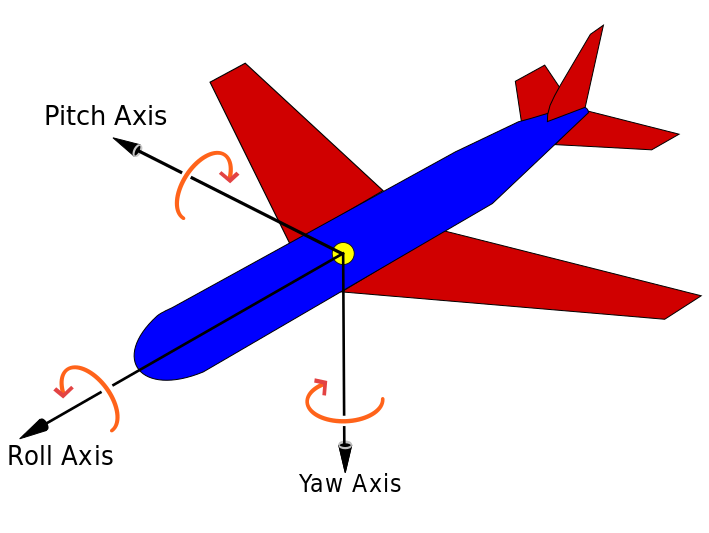
\includegraphics[scale=0.3]{Yaw_Axis_Corrected.png}
    \centering
    \caption{Na rysunku widać położenie trzech osi obrotu: $Ox$, $Oy$ i $Oz$ wraz z towarzyszącymi im kątami. Źródło: \url{https://pl.wikipedia.org/wiki/Macierz_obrotu} [Dostęp: 11.01.22]}
\end{figure}



% \subsection{ Przykłady przekształceń geometrycznych w dwuwymiarowej przestrzeni euklidesowej}

% Do elementarnych przekształceń w dwuwymiarowej przestrzeni euklidesowej ($\mathbb{R}^{2}$) możemy zaliczyć \textit{translację} (przesunięcie), zmianę skali obiektu, bądź jego rotację \citep[s. 2]{Glowacki2013}.

% W przypadku translacji danemu punktowi A w $\mathbb{R}^{2}$ postaci: $A(x_{1}, y_{2})$ przyporządkowuje się nową pozycję poprzez dodanie do współrzędnych punktu A wielkość przesunięcia ($d_{x}$). W wyniku tego otrzymujemy nowy punkt A' postaci: A'($x'_{1}, y'_{2}$). Przedstawiono to na rysunku poniżej.


% \begin{figure}[H]
% 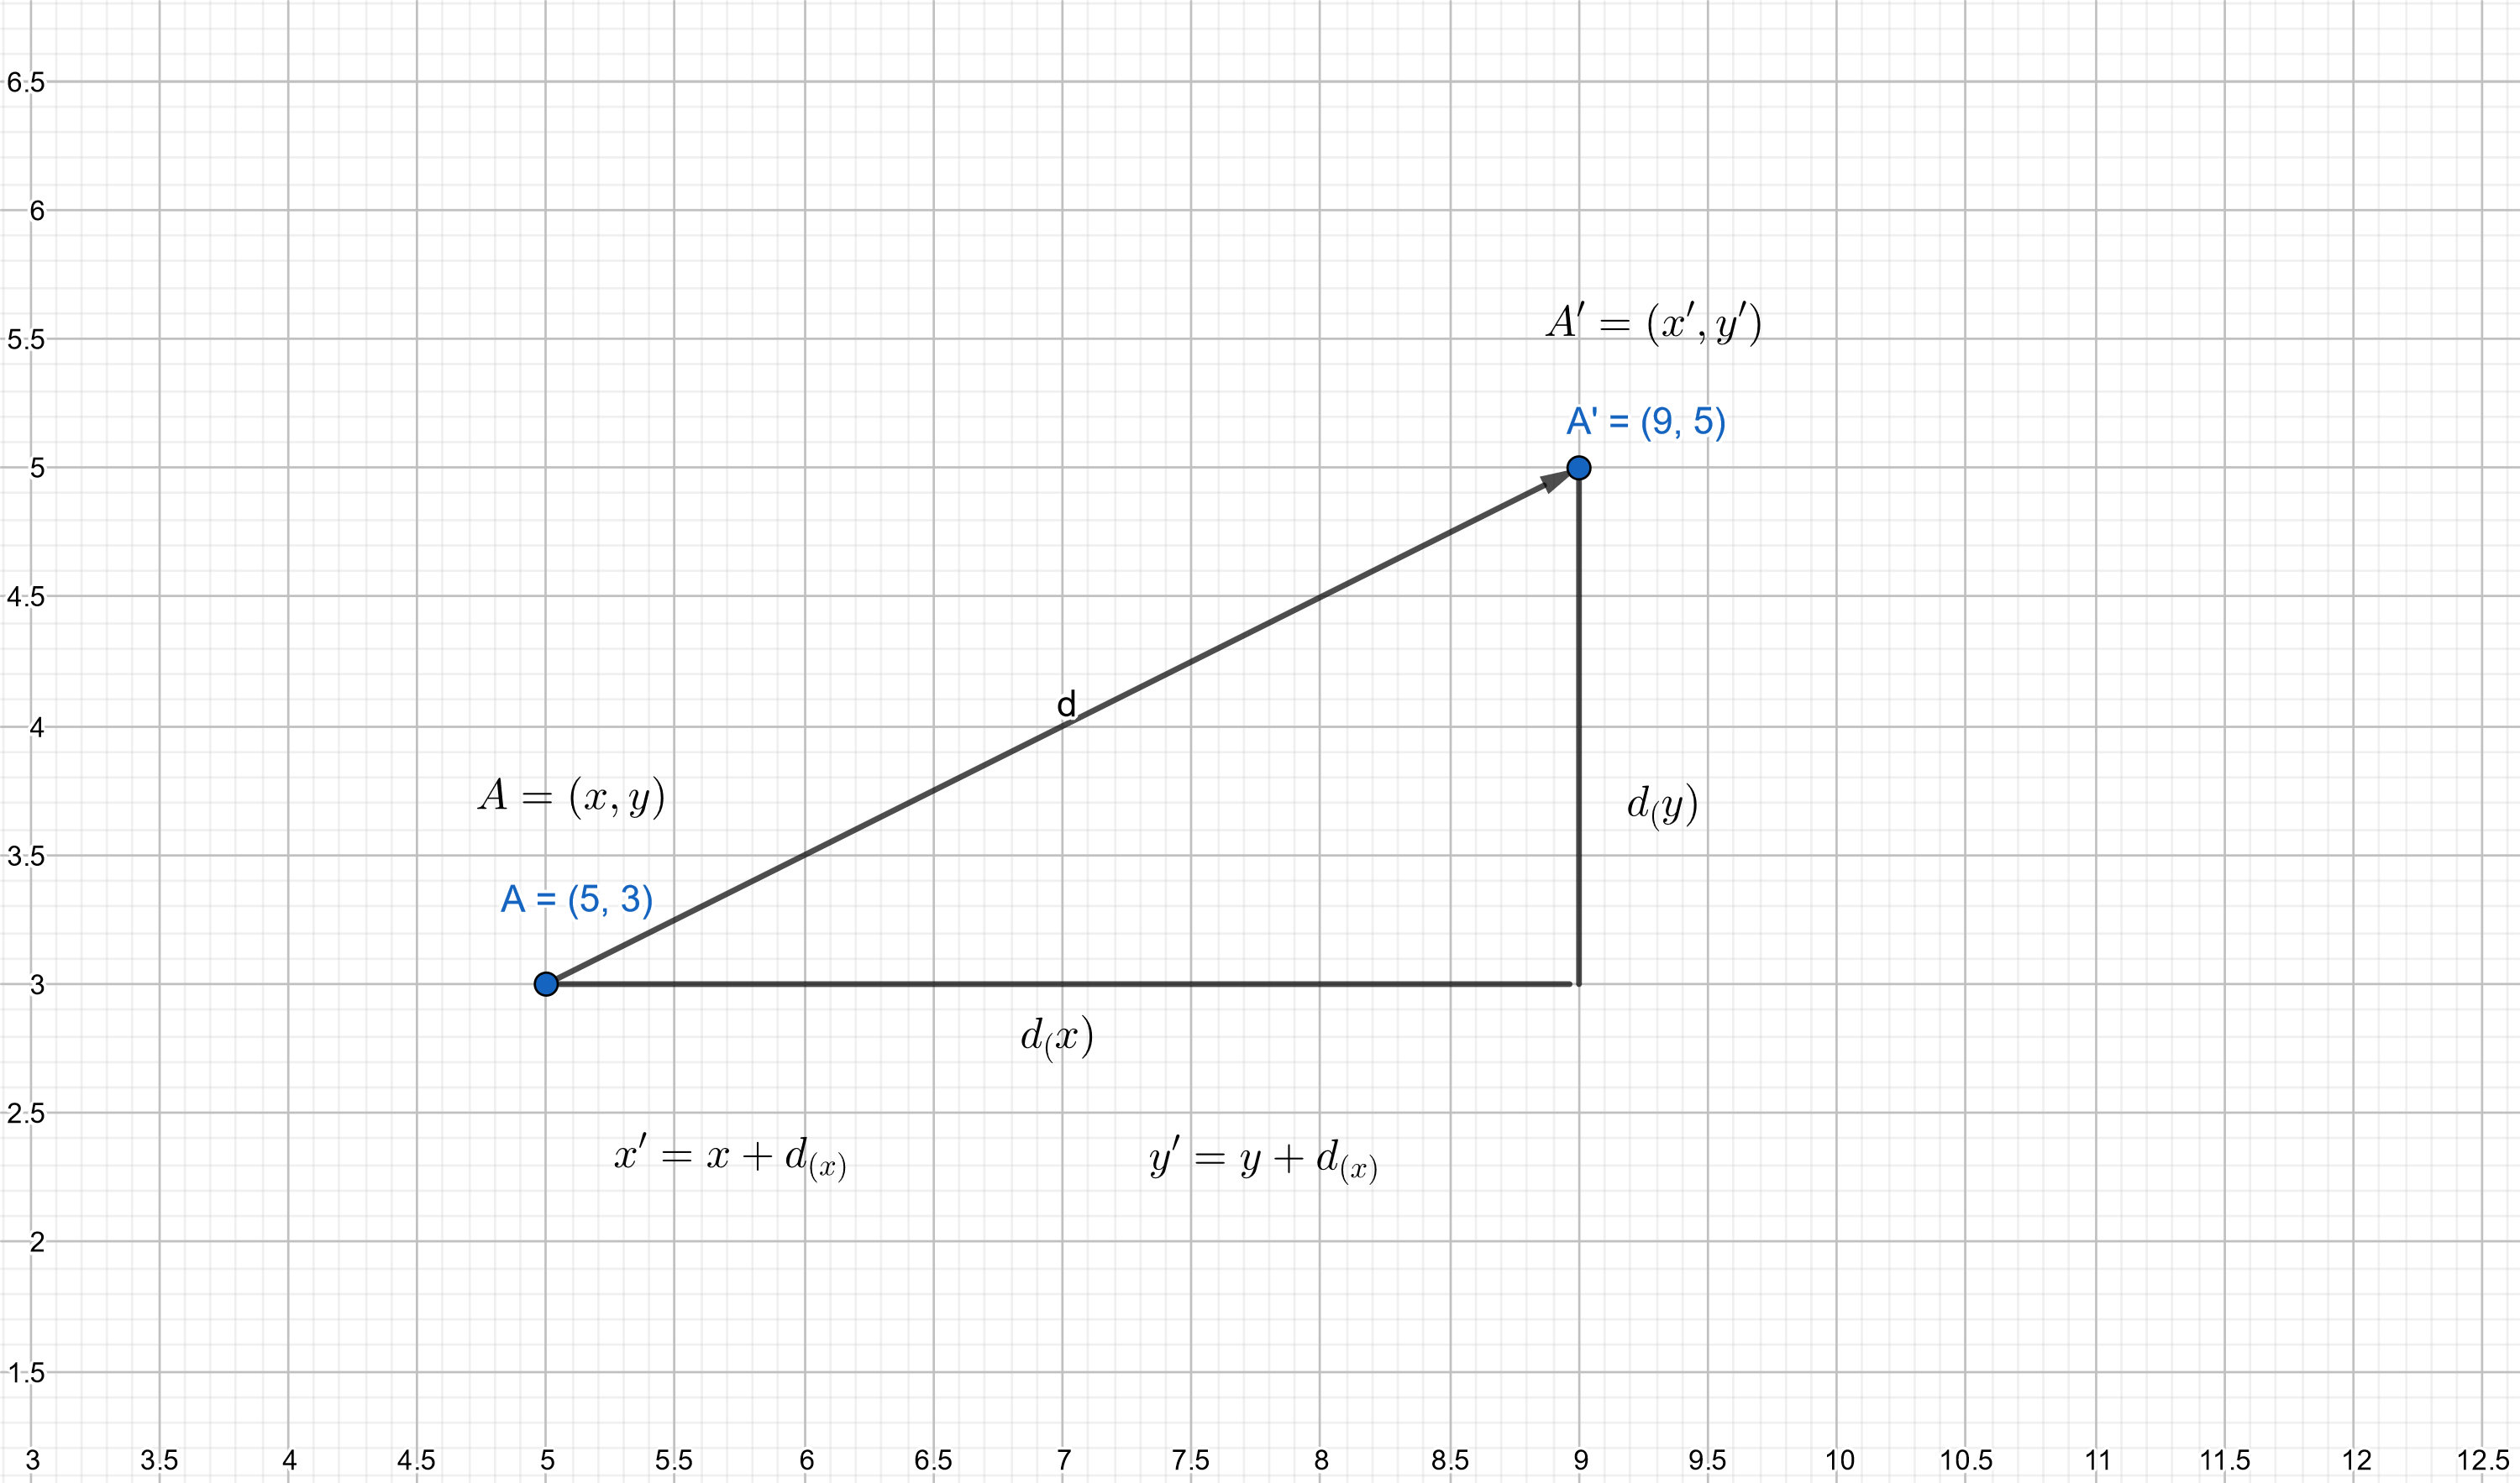
\includegraphics[width=\textwidth]{przesuniecie.png}
% \caption{Przesunięcie punktu $A(5,3)$ do $A'(9,5)$ w dwuwymiarowej przestrzeni euklidesowej $\mathbb{R}^{2}$. Rysunek wykonano za pomocą programu GeoGebra. Źródło: Opracowanie własne na podstawie \citep[s. 4]{Badura2005} i \citep[s. 3]{Glowacki2013}}
% \centering
% \end{figure}

% Skalowanie jest operacją modyfikującą proporcję obrazu względem początku układu współrzędnych. Polega na przesunięciu obiektu względem dowolnie wybranego stałego punktu. Jest nim zwykle początek układu współrzędnych, czyli punkt $(0,0)$. Ten rodzaj skalowania nazywamy \textit{skalowaniem względem początku układu współrzędnych}.

% Obiekty geometryczne można skalować przy za pomocą współczynników $s_{x} \neq 0$ w kierunku osi $OX$ i $s_{y} \neq 0$ w kierunku osi $OY$. Skalowanie względem początku układu współrzędnych to inaczej transformacja odwzorowująca dowolnie wybrany punkt $P(x,y)$ na punkt $P'(x',y')$ przez pomnożenie współrzędnych $x$ i $y$ punktu $P$ przez stałe, niezerowe współczynniki skalowania $s_{x}$ i $s_{y}$.

% Współczynnik skalowania s może zwiększać odległość obiektu względem punktu $(0,0)$ jeśli zachodzi nierówność $|s| > 1$ lub zmniejszać tę odległość jeśli $|s| < 1$. Natomiast jeśli $s_{x} = s_{y}$ to skalowanie nazywamy \textit{jednorodnym}. W przeciwnym wypadku, czyli $s_{x} \neq s_{y}$ skalowanie nazywamy niejednorodnym.

% Jeśli zdecydujemy się przedstawić współrzędne punktów $P$ i $P'$ jako wektory kolumnowe to skalowanie może się odbyć jako mnożenie macierzy przez macierz. Współrzędne punktu $P$ możemy wtedy zapisać wzorami jako:

% \begin{equation*}
%     \begin{bmatrix}
%     x' \\
%     y'
%     \end{bmatrix}
%     =
%     \begin{bmatrix}
%     s_{x} & 0 \\
%     0 & s_{y}
%     \end{bmatrix}
%     \cdot
%     \begin{bmatrix}
%     x \\
%     y
%     \end{bmatrix}
% \end{equation*}

% Macierz:
% \begin{equation*}
% S(s_{x}, s_{y}) =
%     \begin{bmatrix}
%     s_{x} & 0 \\
%     0 & s_{y}
%     \end{bmatrix}
% \end{equation*}

% nazywamy \textit{macierzą skalowania}. Uogólniając powyższe operacje możemy zapisać, że:
% \begin{equation*}
%     P' = S(s_{x}, s_{y}) \cdot P
% \end{equation*}
% \citep[s. 4-5]{Badura2005}.

% Przykład przedstawiono na rysunku poniżej.

% \begin{figure}[H]
% 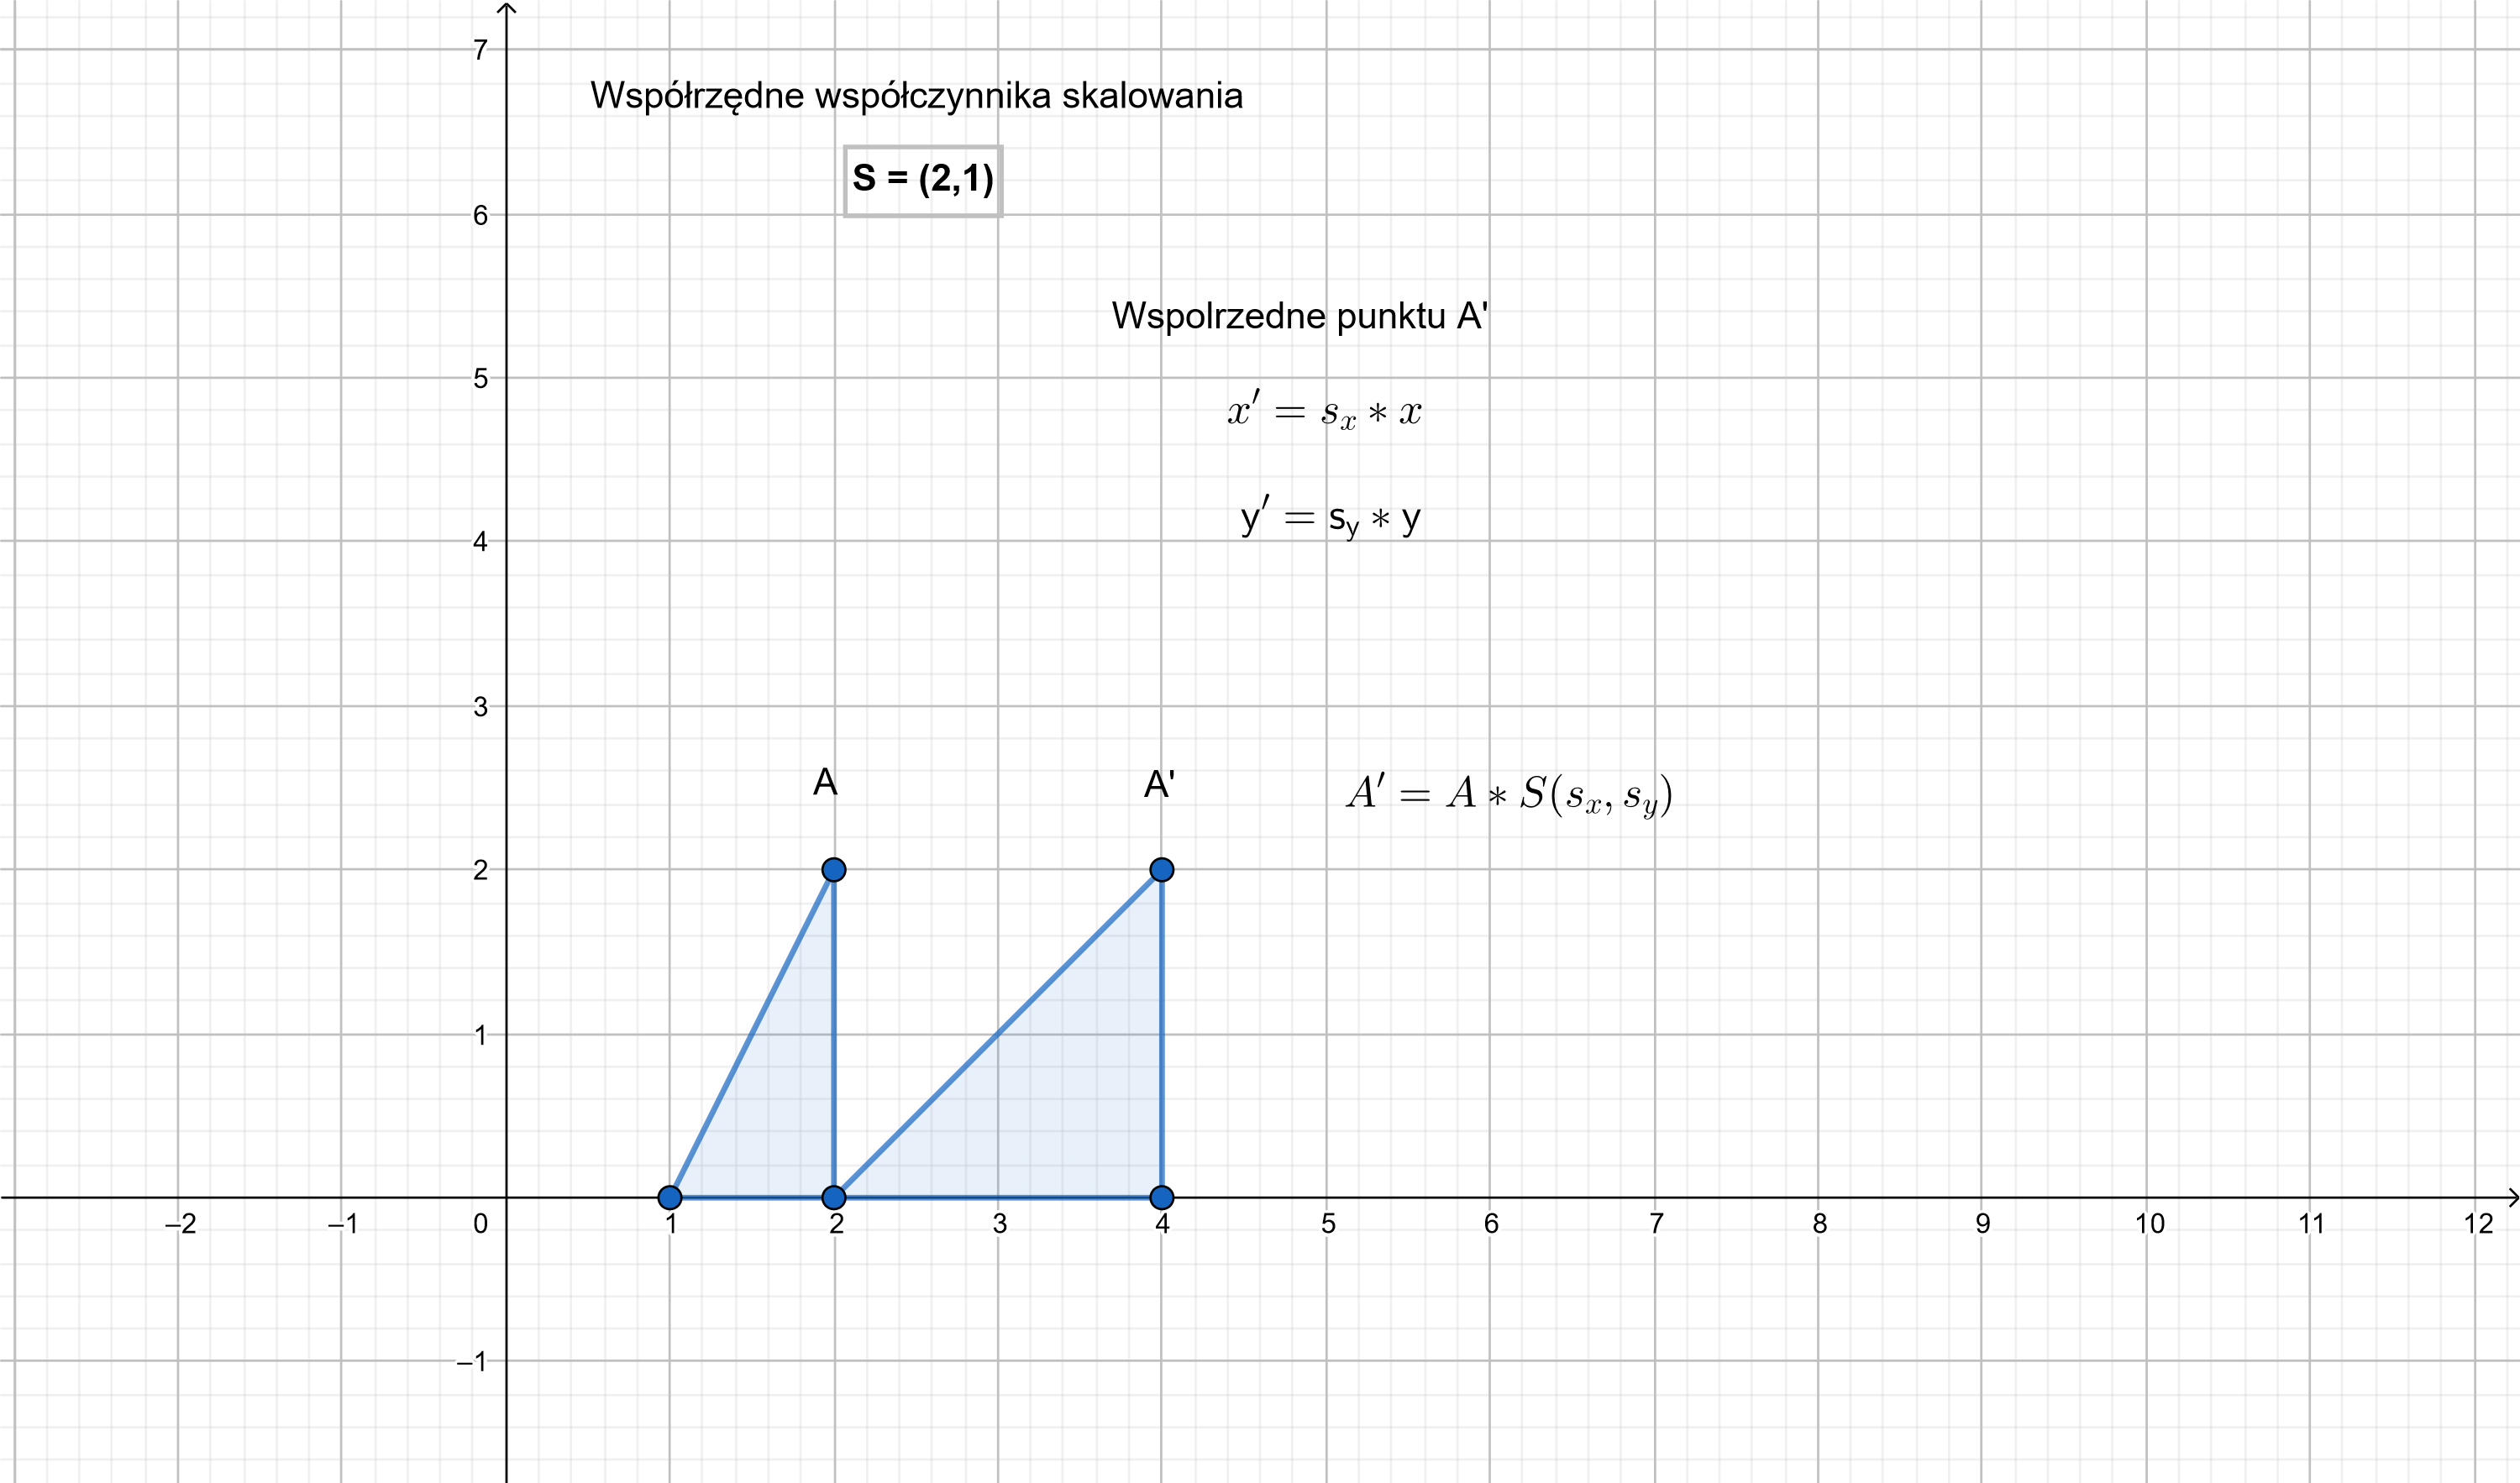
\includegraphics[width=\textwidth]{skalowanie.png}
% \caption{Skalowanie trójkąta A do trójkąta A' względem początku układu współrzędnych i S(2,1). Rysunek wykonano za pomocą programu GeoGebra. Źródło: Opracowanie własne na podstawie \citep[s. 4-5]{Badura2005}} 
% \centering
% \end{figure}

% Ostatnią z operacji jaką chciałbym opisać są obroty figur w $\mathbb{R}^{2}$. Wyróżniamy obroty względem początku układu współrzędnych lub wokół punktu.

% Obrót względem początku układu współrzędnych to operacja polegająca na obrocie poszczególnych punktów obiektu o odgórnie ustalony kąt $\phi$.

% Formalnie obrotem wokół początku układu współrzędnych nazywamy przekształcenie odwzorowujące punkt $P(x,y)$ na punkt $P'(x',y')$ w taki sposób, że odległości punktów $P$ i $P$' od początku układu współrzędnych $O$ spełniają równość $\overline{|OP|} = \overline{|OP'|}$, a kąt między odcinkami $\overline{OP}$ i  $\overline{OP'}$ jest równy wartości kąta $\phi$. Ponieważ istnieją dwa możliwe obrazy punktu $P$ spełniające powyższe warunki przyjęło się, że obrót o kąt dodatni wykonuje się w kierunku przeciwnym do ruchu wskazówek zegara \citep[s. 5 - 6]{Badura2005}.

% Współrzędne Punktu P dane są wzorami:
% \begin{equation}
%     x' = x\cos\phi - y\sin\phi, \quad y' = x\sin\phi + y\cos\phi
% \end{equation}

% Obrót wokół początku układu współrzędnych o kat $\phi$ można wyrazić za pomocą macierzy
% \begin{equation*}
%     \begin{bmatrix}
%     x' \\
%     y'
%     \end{bmatrix}
%     = 
%     \begin{bmatrix}
%     \cos\phi & -\sin\phi \\
%     \sin\phi & \cos\phi
%     \end{bmatrix}
%     \cdot
%     \begin{bmatrix}
%     x \\
%     y
%     \end{bmatrix}
% \end{equation*}
% \\
% Poniższa macierz:
% \begin{equation*}
%     R(\phi) = 
%     \begin{bmatrix}
%     \cos\phi &  -\sin\phi \\
%     \sin\phi & \cos\phi
%     \end{bmatrix}
% \end{equation*}

% Jest \textit{macierzą obrotu}. Opisuje ona  obrót danego wektora (punktu) w przestrzeni $\mathbb{R}^{2}$.
% Zadanie obrotu Punktu P wokół początku układu współrzędnych możemy krótko zapisać jako:
% \begin{equation*}
%     P' = R(\phi) \cdot P
% \end{equation*}

% Obrót wokół początku układu współrzędnych o kąt $\phi$ i odpowiadającą temu obrotowi macierz R będziemy oznaczać poprzez zapis $R(\phi)$ \citep[s. 6-7]{Badura2005}.

% Przykład przedstawiono na poniższym rysunku.

% \begin{figure}[H]
% 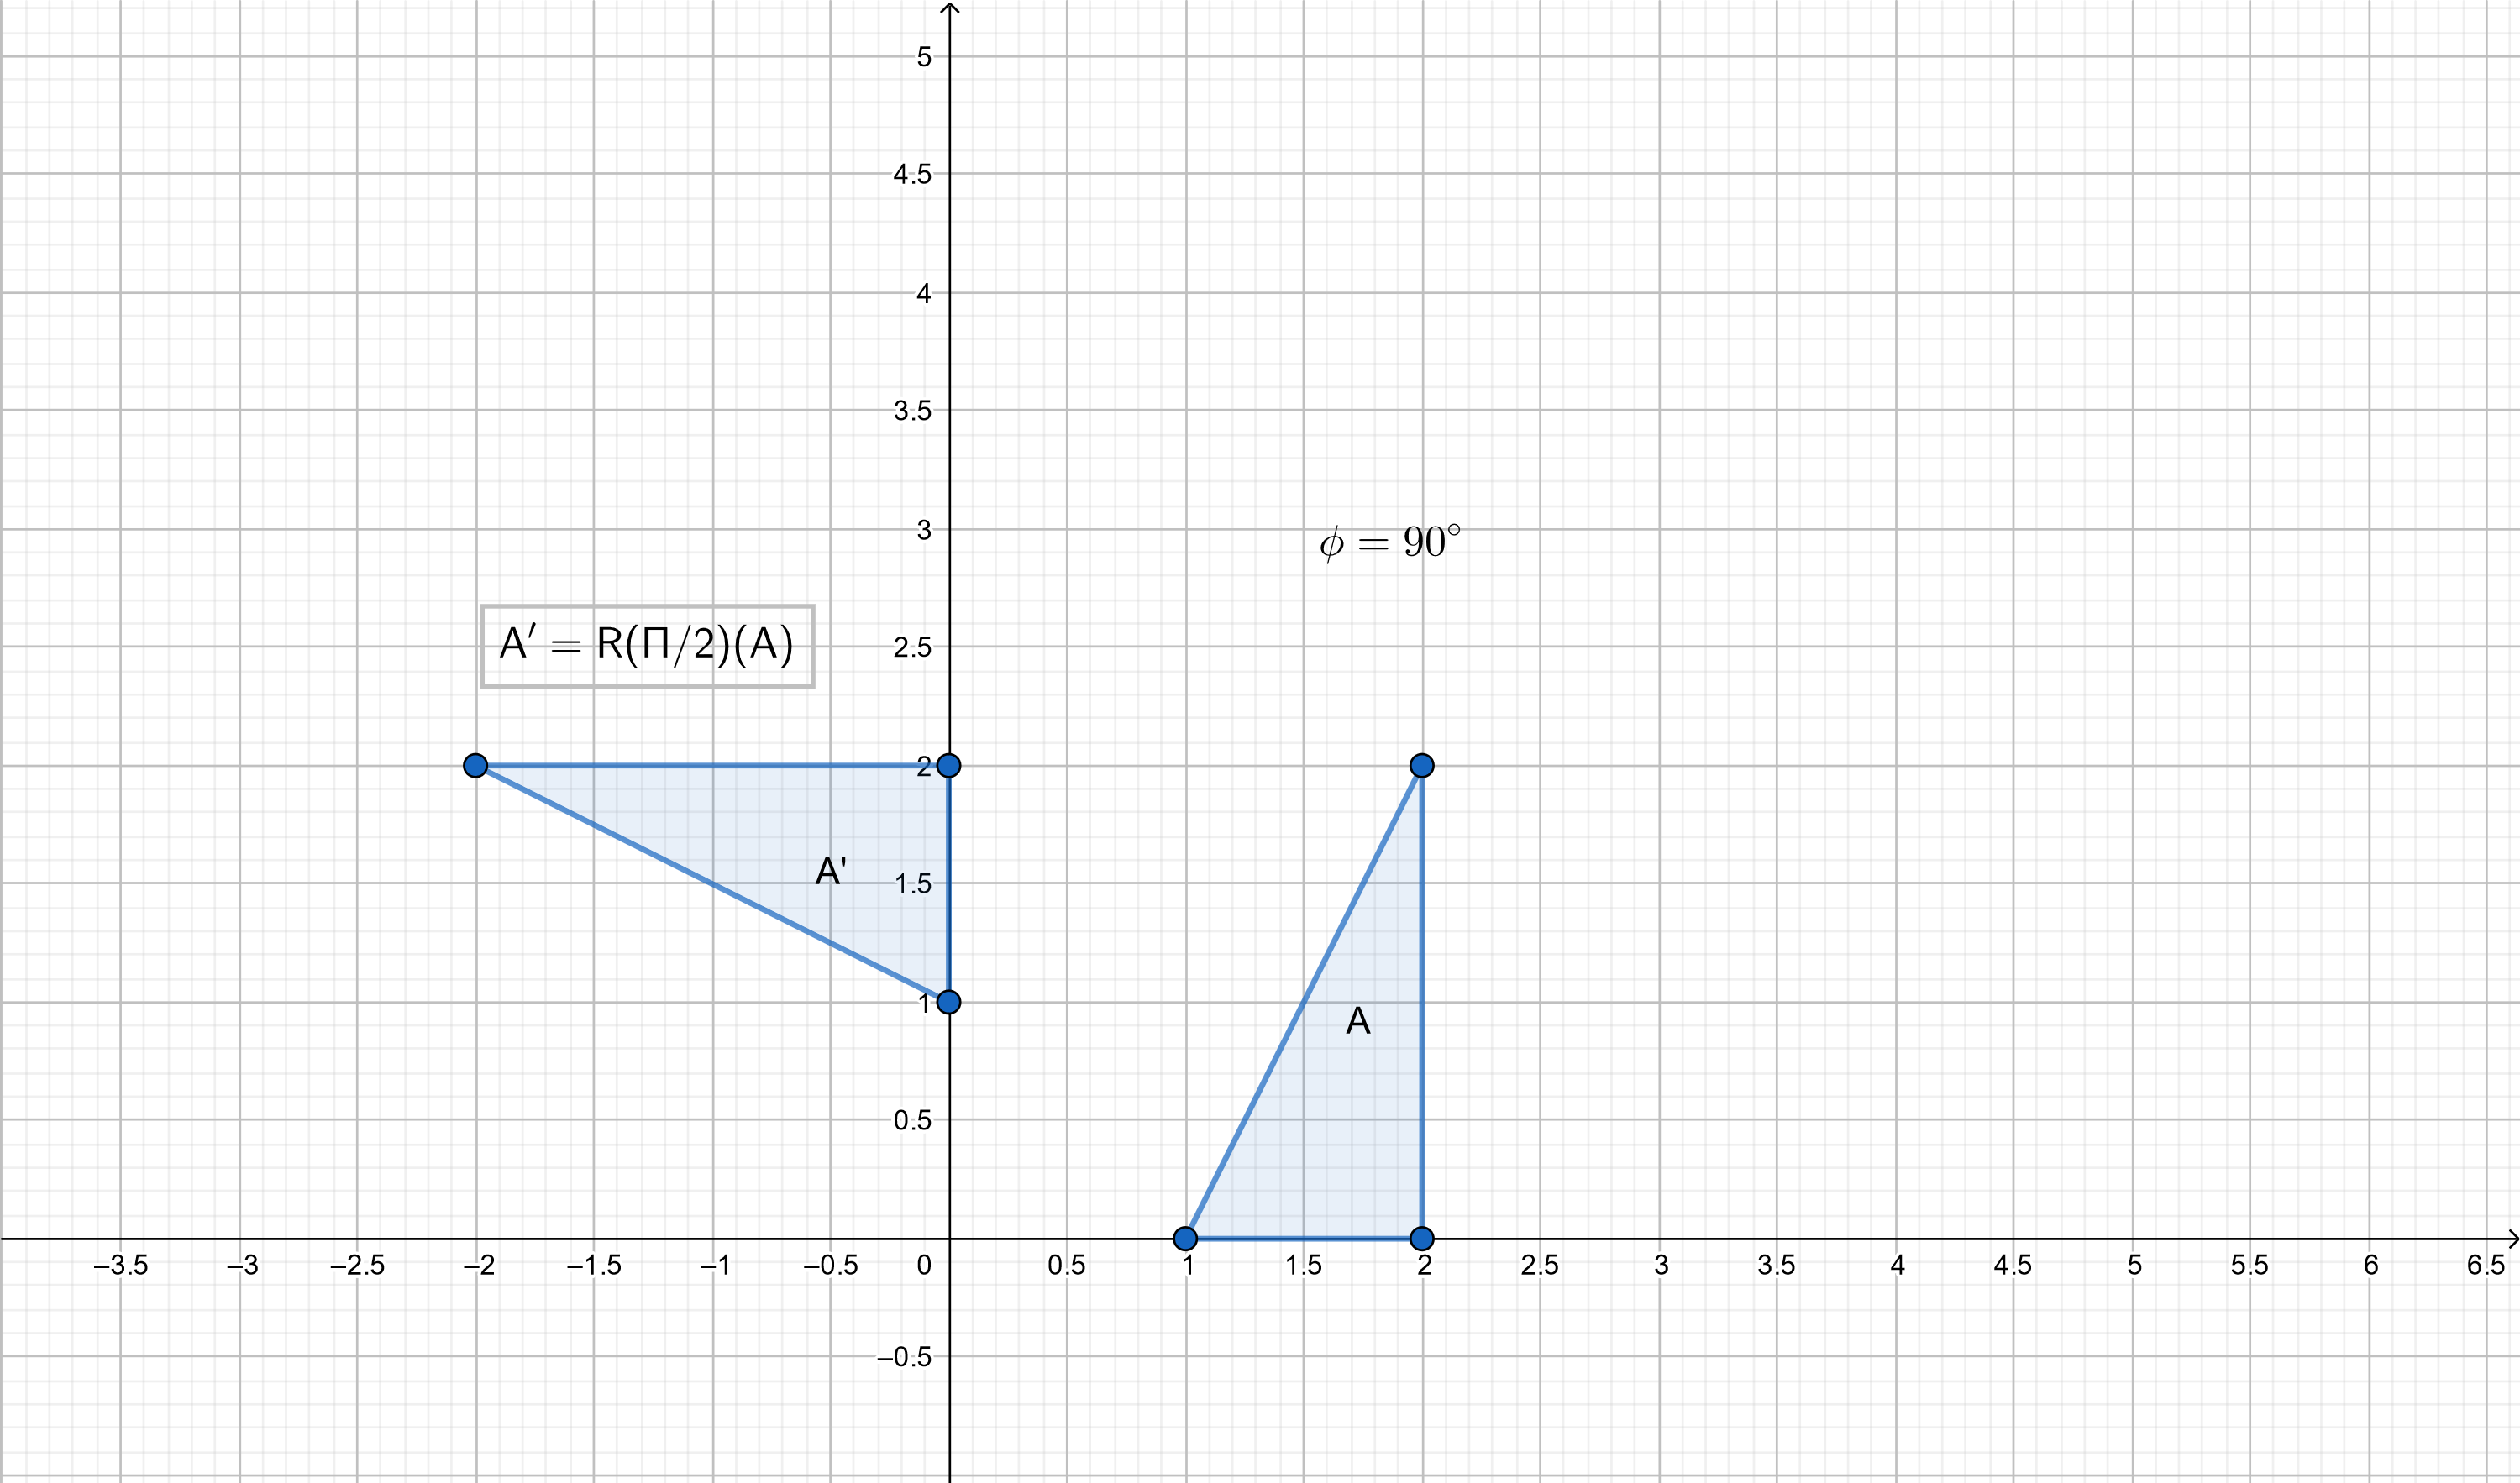
\includegraphics[width=\textwidth]{obrot.png}
% \caption{Obrót trójkąta $A$ do trójkąta $A'$ względem początku układu współrzędnych o kąt $90^{\circ}$. Rysunek wykonano za pomocą programu GeoGebra. Źródło: Opracowanie własne na podstawie \citep[s. 6-7]{Badura2005}} 
% \centering
% \end{figure}


% \subsubsection{Obrót wokół dowolnego punktu}

% Mając do dyspozycji Punkt P o współrzędnych ($x_{0}$ i $y_{0}$)  i jakiś dowolny obiekt możemy spróbować obrócić go wokół punktu $P$ o kąt $\phi$.
% Aby to wykonać potrzebujemy wykonać sekwencyjnie trzy przekształcenia:

% \begin{enumerate}
%     \item Przesunąć punkt $P$ na początek układu współrzędnych,
%     \item Obrót wokół początku układu współrzędnych o podany kąt $\phi$,
%     \item Ponowne przesunięcie płaszczyzny w taki sposób żeby Punkt $P$ powrócił do swojego położenia wyjściowego.
% \end{enumerate}

% Zatem wykonujemy najpierw przesunięcie o wektor $[-x_{0}, -y_{0}]$ aby następnie wykonać obrót wokół początku układu współrzędnych. Na koniec przesuwamy ponownie punkt P o $[x_{0}, y_{0}]$.
% Zapisując te działania bardziej formalnie dochodzimy do następujących wzorów\footnote{\citep[s. 9 - 10]{Badura2005}.}:

% \begin{equation*}
%     x' = (x - x_{0})\cos\phi - (y - y_{0})\sin\phi + x_{0}
% \end{equation*}
% \begin{equation*}
%     y' = (x - x_{0}\sin\phi + (y - y_{0})\cos\phi + y_{0}
% \end{equation*}

% Obrót wokół dowolnego punktu o współrzędnych ($x_{0}$, $y_{0}$) o kąt $\phi$ będziemy oznaczać przez zapis $R_(x_{0},y_{0})$($\phi$) \citep[s. 10]{Badura2005}.
% \\
% Graficzne rozwiązanie problemu przedstawia poniższy rysunek:

% \begin{figure}[H]
% 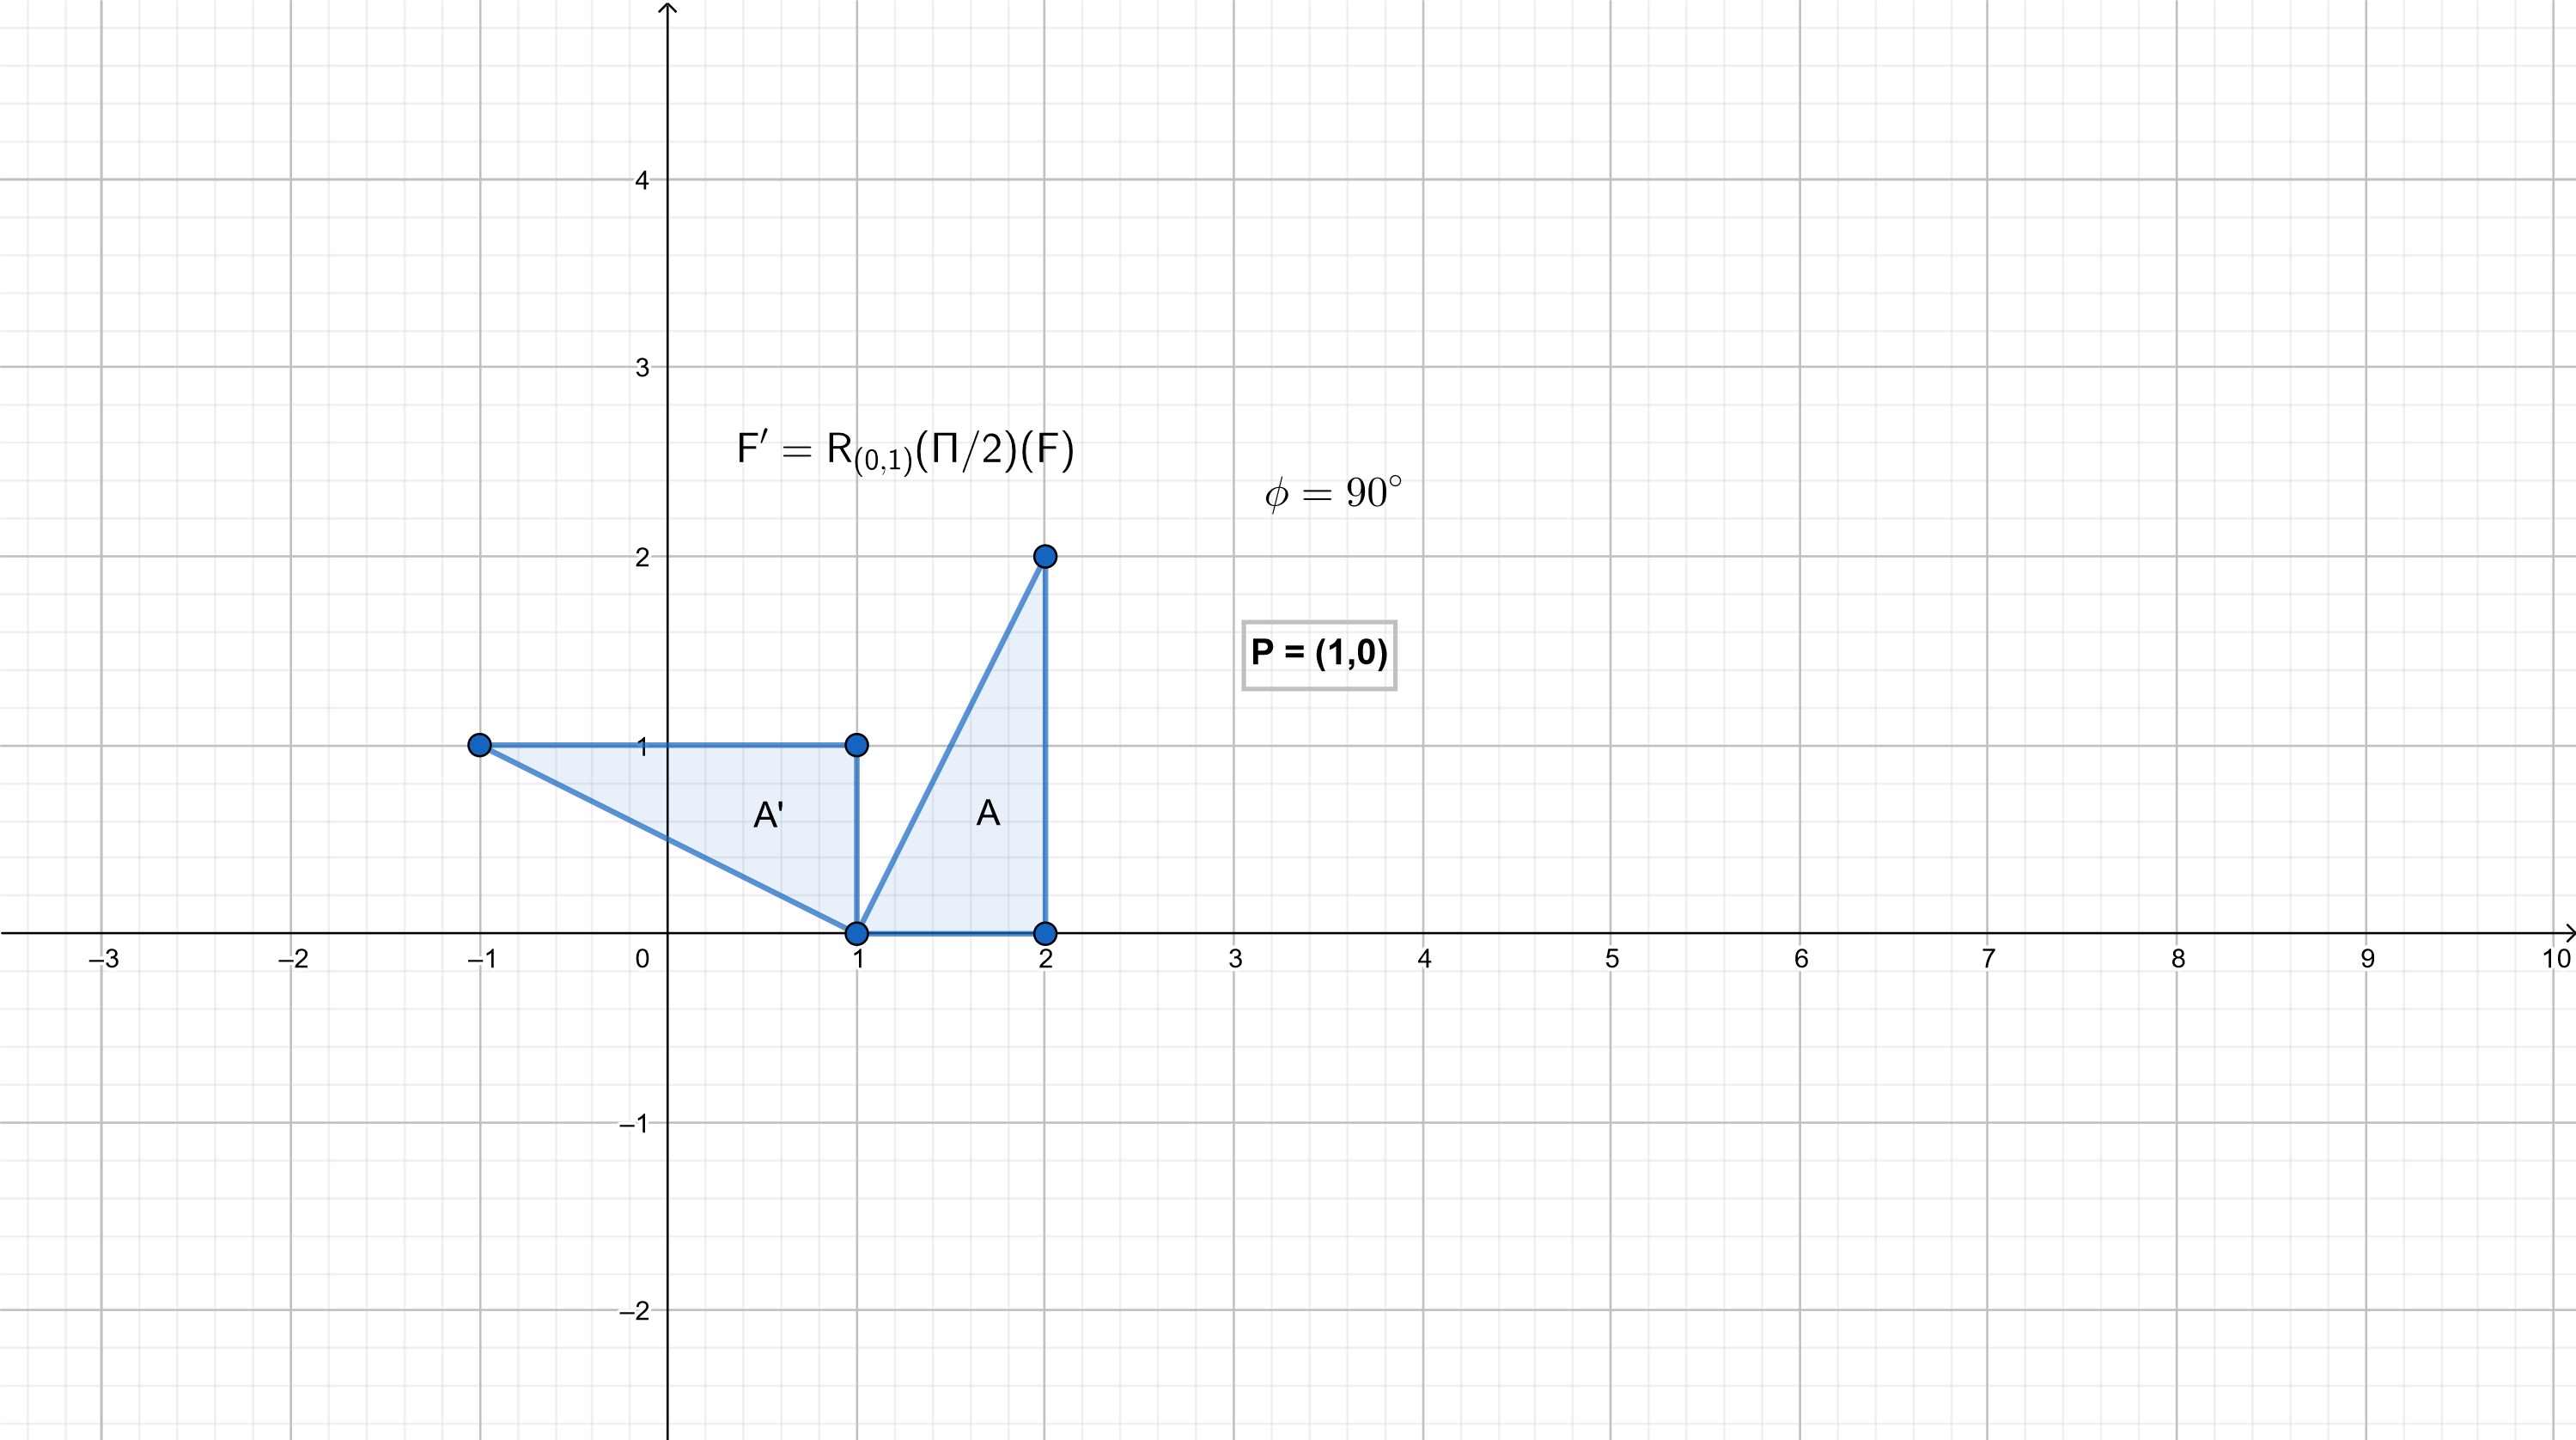
\includegraphics[width=\textwidth]{obrot2.png}
% \caption{Obrót trójkąta $A$ do trójkąta $A'$ względem punktu $P (1,0)$ o kąt $90^{\circ}$. Rysunek wykonano za pomocą programu GeoGebra. Źródło: Opracowanie własne na podstawie \citep[s. 9-10]{Badura2005}} 
% \centering
% \end{figure}
\chapter{Obroty w muzyce}

Wspomniane w poprzednim rozdziale macierze rotacji można wykorzystać do tworzenia muzyki.
W zdefiniowanej w rozdziale pierwszym przestrzeni wektorowej nad ciałem $\mathbb{R}$ możemy rozważyć istnienie  wektorów wartości dźwiękowych (nut) oraz operacje na nich.
Obrót każdego z takich wektorów $v$ gdzie $v \in V$ nad ciałem $\mathbb{R}$ przeprowadzimy za pomocą mnożenia przez macierze obrotu dla osi: $OX$, $OY$ oraz $OZ$. Obroty wektorów zostały zaimplementowane na dwa sposoby:
\begin{enumerate}
    \item Obroty akordów o kąt $5^{\circ}$ w przestrzeni $\mathbb{R}^{3}$,
    \item Obroty wektora nut w przestrzeni $\mathbb{R}^{3}$, reprezentującego własnoręcznie skomponowany utwór w tonacji C-dur, kolejno o kąty $5^{\circ}$, $10^{\circ}$, $15^{\circ}$ oraz $20^{\circ}$ stopni.
\end{enumerate}

\section{Obroty akordów w \texorpdfstring{$\mathbb{R}^{3}$}{R3}}
Na potrzeby eksperymentu przygotowano pogrupowane parami wektory od $v_{1}$ do $v_{4}$ następującej postaci:
\begin{equation*}
v_{1} =
    \begin{bmatrix}
     60 \\
     64 \\
     67
    \end{bmatrix}
    \quad
    v_{2} =
    \begin{bmatrix}
     69 \\
     61 \\
     64
    \end{bmatrix}
    \quad
    v_{3} =
    \begin{bmatrix}
     67 \\
     71 \\
     62
    \end{bmatrix}
    \quad
    v_{4} =
    \begin{bmatrix}
     65 \\
     69 \\
     60
    \end{bmatrix}
\end{equation*}
Następnie każdy z tych wektorów przemnożono przez macierze obrotu odpowiadające poszczególnym osiom $OX$, $OY$ oraz $OZ$ przestrzeni $\mathbb{R}^{3}$:

\begin{equation*}
R_{x}(\alpha) =
    \begin{bmatrix}
    1 & 0 & 0 \\
    0 & \cos\alpha & -\sin\alpha \\
    0 & \sin\alpha & \cos\alpha 
    \end{bmatrix}
    \end{equation*}
    \\
    \begin{equation*}
    R_{y}(\beta) =
    \begin{bmatrix}
    \cos\beta & 0 & \sin\beta \\
    0 & 1 & 0  \\
    -\sin\beta & 0 & \cos\beta
    \end{bmatrix}
    \end{equation*}
    \\
    \begin{equation*}
        R_{z}(\gamma) =
        \begin{bmatrix}
        \cos\gamma & -\sin\gamma & 0 \\
        \sin\gamma & \cos\gamma  & 0 \\
        0 & 0 & 1
        \end{bmatrix}
    \end{equation*}
    Macierz całego obrotu w $\mathbb{R}^{3}$ wyznacza się poprzez pomnożenie wektora $v$ kolejno przez macierze poszczególnych osi, tj.
    \begin{equation*}
        R = R_{x}(\alpha) \cdot R_{y}(\beta) \cdot R_{z}(\gamma).
    \end{equation*}
gdzie kąt $\alpha$ odpowiada rotacji wokół osi $OX$, kąt $\beta$ odpowiada rotacji wokół osi $OY$, a kąt $\gamma$ odpowiada rotacji wokół osi $OZ$. W niniejszym eksperymencie wszystkie wektory obrócono o tę samą wartość, czyli kąt $5^{\circ}$.

\section{Implementacja}
\begin{lstlisting}[language = Haskell]
type Vector = [Double]
type Matrix = [[Double]]

-- macierz obrotu
mx p = [[1,0,0], [0, cos p, sin p], [0, -sin p, cos p]]
my p = [[cos p, 0, - sin p], [0, 1, 0], [sin p, 0, cos p]]
mz p = [[cos p, sin p, 0], [-sin p, cos p, 0], [0, 0, 1]]
-- Dane
-- v1 do v4 to akordy
v1 :: Vector
v1 = [60,64,67]
v2 :: Vector
v2 = [69,61,64]
v3 :: Vector
v3 = [67,71,62]
v4 :: Vector
v4 = [65,69,60]
\end{lstlisting}
Wyznaczenie macierzy całego obrotu w $\mathbb{R}^{3}$:
\begin{lstlisting}[language = Haskell]
-- macierze obrotu 3D
mXY = mmult (mx 5) (my 5) 
mXYZ = mmult (mXY) (mz 5) -- cala macierz obrotu o kat 5
\end{lstlisting}

Funkcja \textit{mmult} służy do mnożenia macierzowego i została zaimplementowana następująco:
\begin{lstlisting}[language = Haskell]
mmult :: Num a => [[a]] -> [[a]] -> [[a]]
mmult a b  = [[sum $ zipWith (*) ar bc | bc <- (L.transpose b)] | ar <- a]
\end{lstlisting}
procedurę obracania wektorów zaimplementowano w poniższy sposób:
\begin{lstlisting}[language = Haskell]
wektor1 = do
    toInt(concat(mmult (w1) mXYZ))
    let nw1 = [80,37,66]
    map pitch nw1
\end{lstlisting}
funkcja \textit{pitch} służy konwersji wartości liczbowych na wartości dźwiękowe.
Następnie do każdego z wektorów dodano ćwierćnuty (qn) za pomocą następującego fragmentu kodu:
\begin{lstlisting}[language = Haskell]
--obrocony wektor 1
rw1 :: [(PitchClass, Octave)]
rw1 = [(Gs,5),(Cs,2),(Fs,4),(G,5),(G,1), (Cs, 5)]
rw1_play :: Music Pitch
rw1_play =  chord $ toMusicPitch qn (rw1)
\end{lstlisting}
Na koniec zaimplementowano monadę umożliwiającą odgrywanie parami oryginalnego akordu wraz z akordem obróconym:

\begin{lstlisting}[language = Haskell]
pierwsza_para :: Music Pitch
pierwsza_para = akord1_music :+: rw1_play

druga_para :: Music Pitch 
druga_para = akord2_music :+: rw2_play

trzecia_para :: Music Pitch 
trzecia_para = akord3_music :+: rw3_play

czwarta_para :: Music Pitch
czwarta_para = akord4_music :+: rw4_play

-- granie wszystkich par
test :: IO ()
test = do
    putStrLn "pierwsza para"
    play pierwsza_para
    putStrLn "Druga para"
    play druga_para
    putStrLn "Trzecia Para"
    play trzecia_para
    putStrLn "Czwarta para"
    play czwarta_para
\end{lstlisting}
    
\section{Wyniki}
Przez $v$ oznaczamy oryginalny wektor, a przez $v'$ wektor obrócony o kąt $\phi = 5^{\circ}$ w $\mathbb{R}^{3}$:

\begin{equation*}
v_{1} =
    \begin{bmatrix}
     60 \\
     64 \\
     67
    \end{bmatrix}
    \quad
    v'_{1} =
    \begin{bmatrix}
     80 \\
     37 \\
     66
    \end{bmatrix}
\end{equation*}
\quad
\begin{equation*}
    v_{2} =
    \begin{bmatrix}
     69 \\
     61 \\
     64
    \end{bmatrix}
    \quad
    v'_{2} =
    \begin{bmatrix}
     92 \\
     34 \\
     55
    \end{bmatrix}
\end{equation*}
\quad
\begin{equation*}
    v_{3} =
    \begin{bmatrix}
     67 \\
     71 \\
     62
    \end{bmatrix}
    \quad
    v'_{3} =
    \begin{bmatrix}
     95 \\
     42 \\
     50
    \end{bmatrix}
\end{equation*}
\quad
\begin{equation*}
    v_{4} =
    \begin{bmatrix}
     65 \\
     69 \\
     60
    \end{bmatrix}
    \quad
    v'_{4} =
    \begin{bmatrix}
     93 \\
     41 \\
     48
    \end{bmatrix}
\end{equation*}

\addtocontents{toc}{\protect\enlargethispage{\baselineskip}}
\section{Wnioski}
Wartości każdego z obróconych wektorów od $v_{1}$ do $v_{4}$ zawierają podobne wartości liczbowe co wektory oryginalnych akordów. Wynika z tego lepsza harmoniczność uzyskanych dźwięków  i ich większe podobieństwo do oryginalnych akordów. Taki efekt uzyskaliśmy dzięki obracaniu wektorów o małe wartości kąta $\phi$ w przypadku większych kątów np. kąta $90^{\circ}$ uzyskane dźwięki znacznie różniłyby się od oryginalnych, a przejście pomiędzy oryginałem, a nowo uzyskanym wektorem obróconym byłoby bardziej zauważalne, co odbiłoby się negatywnie na odczuciach estetycznych odbiorcy muzyki i harmonii samego dźwięku.

\addtocontents{toc}{\protect\enlargethispage{\baselineskip}}

\section{Obroty melodii w \texorpdfstring{$\mathbb{R}^{3}$}{R3}}

Jako podstawę utworu bazowego zdefiniowanego w Haskellu następujące tablice dźwięków. Każda z poniższych tablic zawiera 12 dźwięków:
\begin{lstlisting}[language = Haskell]
linia1 = [C, E, G, B, D, F, A, C, E, G, B, C] 
linia2 = [C, F, A, D, G, C, F, B, E, A, D, G] 
linia3 = [C, A, F, D, B, G, E, C, A, F, D, B]
linia4 = [C, G, E, B, G, D, B, F, D, A, F, C] 
\end{lstlisting}
Następnie do każdej z tablic dołączono nuty. Funkcja \textit{pcToQN} dołącza ćwierćnuty, natomiast funkcja \textit{pcToHN} dołącza półnuty:
\begin{lstlisting}[language = Haskell]
part1 = map pcToHN (linia1)
part2 =  map pcToQN (linia2)
part3 = map pcToHN (linia3)
part4 =  map pcToQN(linia4)
\end{lstlisting}
Ostatni krok to skonwertowanie takiego zapisu w formacie \textit{dźwięk -- długość} na typ muzyczny \textit{Music Pitch}, co umożliwi odgrywanie utworu. Umożliwia to konstruktor \textit{line \$}:
\begin{lstlisting}[language = Haskell]
part1_music = line $ part1
part2_music = line $ part2
part3_music = line $ part3
part4_music = line $ part4
\end{lstlisting}
Mając skomponowany utwór, przystępujemy do jego obrotu w przestrzeni $\mathbb{R}^{3}$. W tym celu każda z linii melodycznych skonwertowaliśmy na wektory:
\begin{lstlisting}[language = Haskell]
v1 :: Vector
v1 = [0,4,7,11,2,5,9,0,4,7,11,0]
v2 :: Vector
v2 =[0,5,9,2,7,0,5,11,4,9,2,7]
v3 :: Vector
v3 = [0,9,5,2,11,7,4,0,9,5,2,11]
v4 :: Vector
v4 =[0,7,4,11,7,2,11,5,2,9,5,0]
\end{lstlisting}
Dzięki temu można wykonać operacje przemnożenia poprzez macierze obrotu osi $OX$, $OY$ i $OZ$, analogiczne do przedstawionych wcześniej.
Obrót zaimplementowano następująco:
\begin{lstlisting}[language = Haskell]
--obracanie wektorow
wektor1 = do
    toInt(concat(mmult (w1) mXYZ))
    

wektor2 = do
    toInt(concat(mmult (w2) mXYZ))
    
wektor3 = do
    toInt(concat(mmult (w3) mXYZ))
    

wektor4 = do
    toInt(concat(mmult (w4) mXYZ))
\end{lstlisting}

Każdy pojedynczy obrót umożliwiał uzyskanie nowego wektora trójwymiarowego. Dla wektorów $v_{1}$, $v_{2}$, $v_{3}$ i $v_{4}$ przy przykładowym obrocie o kąt $\phi = 20^{\circ}$ uzyskaliśmy kolejno:
\begin{equation*}
v'_{1} =
\begin{bmatrix}
7 \\
3 \\
3
\end{bmatrix}
\quad
v'_{2} =
\begin{bmatrix}
9 \\
4 \\
3
\end{bmatrix}
\quad
v'_{3} =
\begin{bmatrix}
5 \\
8 \\
4
\end{bmatrix}
\quad
v'_{4} =
\begin{bmatrix}
4 \\
6 \\
3
\end{bmatrix}
\end{equation*}
W tej procedurze testowej każdy kolejny obrót wykonywaliśmy o inny kąt, chcąc sprawdzić, czy także tym razem uzyskany utwór wynikowy będzie podobny do oryginalnego.
Składając wszystkie próby razem uzyskaliśmy utwór o długości 12 dźwięków, dokładnie tak jak w utworze oryginalnym:
\begin{lstlisting}[language = Haskell]
-- 1. Obrot o 5 stopni
rotate1 = [8,1,1,10,1,1,9,5,2,7,3,2] --linia1
-- 2. o 10 stopni
rotate2 = [3,3,7,4,4,9,7,1,8,5,1,6] -- linia2
-- 3. o 15 stopni
rotate3 = [6,5,2,8,6,3,6,9,2,4,7,1] -- linia3
-- 4. o 20 stopni 
rotate4 = [7,3,3,9,4,3,5,8,4,4,6,3] --linia4
\end{lstlisting}

Następująca monada umożliwia odgrywanie utworu oryginalnego razem z obróconym:
\begin{lstlisting}[language = Haskell]
test :: IO ()
test = do
    putStrLn "pierwszy utwor" 
    play utwor
    putStrLn "Ten sam utwor, ale po obrocie"
    play rotate_utwor
\end{lstlisting}

\addtocontents{toc}{\protect\enlargethispage{\baselineskip}}

\section{Wnioski}
Nowo uzyskany utwór zachował harmonie oryginalnego utworu, a uzyskane dźwięki wydają się podobne do oryginału. Wynika z tego następujący wniosek: Jeżeli obracamy utwór w przestrzeni nad ciałem $\mathbb{R}^{3}$, to podobnie jak w przypadku akordów należy to uczynić o małe wartości kątów, gdyż zwiększa to prawdopodobieństwo tego, że uzyskane dźwięki będą brzmieniowo zbliżone do oryginału. Nie musimy jednak  obracać utworu cały czas o ten sam kąt -- mogą to być inne wartości kątów o ile ich wartości nie są zbyt duże.
\chapter*{Zakończenie}
\noindent Celem pracy było pokazanie jak duży potencjał tkwi w metodach uczeniach maszynowego takich jak sieci neuronowe. Okazuje się, że tak klasyczny problem algorytmiczny jak klasyfikacja obiektu do jednej z predefiniowanej klasy może umożliwić rozwój dziedzin zupełnie niezwiązanych z informatyką, takich jak tworzenie muzyki -- będącej jak dotychczas niepodzielnym królestwem człowieka. Maszyna, jeżeli dobrze się ją zaprogramuje, potrafi rozpoznawać utwory muzyczne równie dobrze jak człowiek. 
Jednak potencjał metod numerycznych nie ogranicza się jedynie do zadań rozpoznawania. Maszyna jest zdolna także do komponowania muzyki. Metoda, którą tutaj pokazaliśmy ma wiele ograniczeń, ale na pewno istnieje w niej pewien potencjał, który jest warty poznania i dalszych rozważań, do których niniejsza praca miała zachęcić.

\bibliographystyle{unsrt}
\bibliography{bibliography}
\end{document}

